% Format teze zasnovan je na paketu memoir
% http://tug.ctan.org/macros/latex/contrib/memoir/memman.pdf ili
% http://texdoc.net/texmf-dist/doc/latex/memoir/memman.pdf
% 
% Prilikom zadavanja klase memoir, navedenim opcijama se podešava 
% veličina slova (12pt) i jednostrano štampanje (oneside).
% Ove parametre možete menjati samo ako pravite nezvanične verzije
% mastera za privatnu upotrebu (na primer, u b5 varijanti ima smisla 
% smanjiti 
\documentclass[12pt,oneside]{memoir}

% Paket koji definiše sve specifičnosti mastera Matematičkog fakulteta
\usepackage[latinica]{matfmaster}
%
% Podrazumevano pismo je ćirilica.
%   Ako koristite pdflatex, a ne xetex, sav latinički tekst na srpskom jeziku
%   treba biti okružen sa \lat{...} ili \begin{latinica}...\end{latinica}.
%
% Opicija [latinica]:
%   ako želite da pišete latiniciom, dodajte opciju "latinica" tj.
%   prethodni paket uključite pomoću: \usepackage[latinica]{matfmaster}.
%   Ako koristite pdflatex, a ne xetex, sav ćirilički tekst treba biti
%   okružen sa \cir{...} ili \begin{cirilica}...\end{cirilica}.
%
% Opcija [biblatex]:
%   ako želite da koristite reference na više jezika i umesto paketa
%   bibtex da koristite BibLaTeX/Biber, dodajte opciju "biblatex" tj.
%   prethodni paket uključite pomoću: \usepackage[biblatex]{matfmaster}
%
% Opcija [b5paper]:
%   ako želite da napravite verziju teze u manjem (b5) formatu, navedite
%   opciju "b5paper", tj. prethodni paket uključite pomoću: 
%   \usepackage[b5paper]{matfmaster}. Tada ima smisla razmisliti o promeni
%   veličine slova (izmenom opcije 12pt na 11pt u \documentclass{memoir}).
%
% Naravno, opcije je moguće kombinovati.
% Npr. \usepackage[b5paper,biblatex]{matfmaster}

% Pomoćni paket koji generiše nasumičan tekst u kojem se javljaju sva slova
% azbuke (nema potrebe koristiti ovo u pravim disertacijama)
\usepackage{pangrami}
\usepackage[x11names]{xcolor}
%\usepackage{roboto}
\usepackage{courier}
\usepackage{numprint}

% Paket koji obezbeđuje ispravni prikaz ćiriličkih italik slova kada
% se koristi pdflatex. Zakomentarisati ako na sistemu koji koristite ovaj
% paket nije dostupan ili ako ne radi ispravno.
\usepackage{cmsrb}
\usepackage{graphicx}
\usepackage{subcaption}

% Ostali paketi koji se koriste u dokumentu
\usepackage{listings} % listing programskog koda

% Datoteka sa literaturom u BibTex tj. BibLaTeX/Biber formatu
\bib{matfmaster-primer}

% Ime kandidata na srpskom jeziku (u odabranom pismu)
\autor{Luka B. Đorović}
% Naslov teze na srpskom jeziku (u odabranom pismu)
\naslov{Analiza slučajeva upotrebe relacionih i kolonski orijentisanih nerelacionih baza podataka}
% Godina u kojoj je teza predana komisiji
\godina{2024}
% Ime i afilijacija mentora (u odabranom pismu)
\mentor{др Saša \textsc{Malkov}, vanredni profesor\\ Универзитет у Београду, Математички факултет}
% Ime i afilijacija prvog člana komisije (u odabranom pismu)
\komisijaA{dr Nenad \textsc{Mitić}, redovni profesor\\ Универзитет у Београду, Математички факултет}
% Ime i afilijacija drugog člana komisije (u odabranom pismu)
\komisijaB{dr Ivana \textsc{Tanasijević}, доцент\\ Универзитет у Београду, Математички факултет}
% Ime i afilijacija trećeg člana komisije (opciono)
% \komisijaC{}
% Ime i afilijacija četvrtog člana komisije (opciono)
% \komisijaD{}
% Datum odbrane (obrisati ili iskomentarisati narednu liniju ako datum odbrane nije poznat)
\datumodbrane{}

% Apstrakt na srpskom jeziku (u odabranom pismu)
\apstr{
Специфични циљ рада је анализа и упоређивање случајева употребе релационих и
колонски оријентисаних нерелационих база података. Рад се састојi из теоријског
описа наведених технологија, као и описа конкретних представника база података који ће
бити коришћени.
У раду su на основу теоријских и практичних извора и истраживања,  анализирани различити случајеви употребе. Примери случајева употребе праћени su
експериментима који се састојe од извршавања различитих врста поступака. Razmatrani primeri slučajeva upotrebe su:
primena u transakcionom procesiranju, primena u analitičkom procesiranju kao i primena u distribuiranom okruženju.
}

% Ključne reči na srpskom jeziku (u odabranom pismu)
\kljucnereci{podaci, SQL, NoSQL, BigData, relacioni, kolonski-orijentisani}

\begin{document}
% ==============================================================================
% Uvodni deo teze
\frontmatter
% ==============================================================================
% Naslovna strana
\naslovna
% Strana sa podacima o mentoru i članovima komisije
\komisija
% Strana sa posvetom (u odabranom pismu)
\posveta{Ovaj rad posvećujem...}
% Strana sa podacima o disertaciji na srpskom jeziku
\apstrakt
% Sadržaj teze
\tableofcontents*

% ==============================================================================
% Glavni deo teze
\mainmatter
% ==============================================================================

% ------------------------------------------------------------------------------
\chapter{Uvod}
% ------------------------------------------------------------------------------

Podaci su najstabilniji deo svakog sistema. Oni su reprezentacija činjenica i instrukcija u formalizovanom stanju spremnom za dalju interakciju, interpretaciju ili obradu od strane korisnika ili mašine. Iako kroz svoju istoriju računarstvo važi za oblast koja uvodi nove tehnologije i alate velikom brzinom, to nije slučaj za svaku njenu granu. Postoje oblasti koje se kroz istoriju nisu menjale ili su se slabo menjale i proširivale. Primera za to ima puno i oni su uglavnom usko vezani za funkcionalne principe koji se prožimaju kroz računarske mreže, kompilatore, operativne sisteme, sisteme za upravljanje podacima itd. 

Kada je reč o istoriji sistema za upravljanje podacima mogu se izdvojiti tri faze: period pre relacionih sistema, vreme dominantnog korišćenja relacionih sistema i nastanak alternativa relacionim sistemima pod grupnim nazivom \textit{NoSQL}.

Do nastanka relacionih sistema rukovanje podacima izvodilo se kroz pisanje i čitanje iz datoteka operativnog sistema. Rukovanje većim količinama podataka nije bilo standardizovano ni na koji način, već su se konvencije uvodile na nivou organizacija.  Jedan od primera je i \textit{Apollo} sletanje na Mesec koje je realizovano korišćenjem ovakvog vida rada sa podacima \cite{ColumnarOriented}. 

Međutim, ovaj način rada imao je mnogobrojne mane, među kojima je jedna od glavnih bila komplikovan pristup podacima. To je stvorilo potrebu za daljim istraživanjima i unapređenjem.  Edgar F. Codd\footnote{Edgar Frank "Ted" Codd (19 Avugst 1923 – 18 April 2003) Američki računarski naučnik }  je 1970. godine objavio rad pod imenom "\textit{A Relational Model of Data for Large Shared Data Banks}" kao rezultat sopstvenih istraživanja i teorija o organizaciji podataka. Dokaz da je njegov model moguće implementirati bila je realizacija projekta System R\footnote{System R - sistem za rad sa podacima napravljen kao deo istraživačkog projekta IBM-a}, što je rezultiralo pojavom SQL-a (\textit{Structured Query Language}) kao standardizovanog jezika za rad sa podacima. Nakon toga na tržištu su se pojavili Oracle i IBM sa svojim komercijalnim proizvodima za upravljanje relacionim bazama podataka. Naredni period obeležio je rad sa podacima koristeći relacioni model.  

Ubrzana digitalizacija i povećana dostupnost interneta, donela je sa sobom potrebu za obradom veće količine podataka. Sve ovo je pokazalo pojedine slabosti dosadašnjih sistema zasnovanih na relacionim modelima, koji nisu mogli u svim segmentima da odgovore na zahteve modernog doba. Ovi problemi, poznati pod imenom: problemi velikih podataka (engl \textit{BigData problems}), doveli su do pojave niza novih modela i principa za čuvanje podataka, kojima je dodeljen  grupni naziv: nerelacione baze podataka (engl. \textit{NoSQL}).
Sistematizovanje ogromne količine fizičkog prostora na disku na kojem se podaci mogu čuvati i kasnije koristiti, kao i fleksibilnost strukture podataka sa kojima se radi, glavni su problemi tog vremena na koje su se fokusirale tehnologije nastale u \textit{NoSQL} pokretu.
Decenije vladavine  relacionih sistema za čuvanje podataka ostavile su dubok trag u praksama rada sa podacima, i sa razlogom predstavljaju standard i dan danas, te je eventualno usvajanje tehnologija nastalih u ovoj fazi i dalje  česta dilema mnogih stručnjaka. 

Kao važna grupa nerelacionih baza podataka izdvajaju se kolonski-orijentisane baze podataka. One su uvele tada nekonvencionalne koncepte čuvanja podataka po kolonama. To podrazumeva sekvencijalno skladištenje vrednosti jedne kolone na disku, sa referencom na red kojem pripada. To sa sobom donosi razne mogućnosti za optimizaciju, ali i nove pristupe modelovanja i organizacije podataka. Ovakav način skladištenja ispitivan je još davnih sedamdesetih godina XX veka, međutim u ranim godinama XXI veka došlo je do obnove interesovanja u akademskim,  ali i industrijskim krugovima. 

Nijedan od navedenih koncepata nije univerzalno rešenje, zato je bitno postojanje sadržaja koji se bave analizom slučajeva upotrebe tih tehnologija. Pored teorijske analize, koja se može pronaći u relevantnim javnim dokumentacijama, korisno je imati i konkretne implementacije testova čiji se rezultati mogu iskoristiti kako bi se povukle paralele u skladu sa potrebama realnih  sistema. 

Cilj ovog rada je analiza i upoređivanje slučajeva upotrebe relacionih i kolonski orijentisanih baza podataka. Rad se sastoji iz teorijskog opisa navedenih tehnologija, kao i opisa konkretnih predstavnika baza podataka kojesu korišćeni. Na osnovu teorijskih izvora i istraživanja analizirani su  različiti slučajevi upotrebe. 


% ------------------------------------------------------------------------------
\chapter{Modeli podataka}
\label{chp:razrada}
\section{Relacioni model}
\subsection{Opšte karakteristike}
Relacioni model je najpopularniji model za rad sa podacima. On podatke kao i veze između njih predstavlja kroz skup relacija koje predstaljaju skupove torki. Da bi jedan skup torki ili vrsta bio validna relacija u relacionom modelu, on mora ispunjavati sledeće uslove \cite{ColumnarOriented}:

\begin{enumerate}
\item[\textbullet] Presek kolone i vrste jedinstveno određuje vrednosnu ćeliju.

\item[\textbullet] Sve vrednosne ćelije jedne kolone pripadaju nekom zajedničkom skupu. 

\item[\textbullet] Svaka kolona ima jedinstveno ime.

\item[\textbullet] Ne postoje dve identične vrste jedne relacije. 
\end{enumerate}

Iako ovakva formalizacija relacije jeste intuitivna (usled istorijskog uticaja koji je relacioni model ostavio na ideju organizacije podataka) ona je neophodna za  definisanje složenijih pojmova. 

\subsection{Koncept ključa relacionog modela}

Skup kolona relacije za koji važi da dva reda te relacije nemaju identične vrednosti za svaku kolonu iz tog skupa naziva  se \textit{natključ} relacije. Svaki minimalan natključ je \textit{ključ kandidat}. Svaka relacija može imati više ključeva kandidata, a jedan on njih se bira za  \textit{primarni ključ} koji mora imati definisanu vrednost za svaku njegovu kolonu.
\textit{Strani ključ} je kolona ili skup kolona čije vrednosti predstavljaju referencu na određeni red neke druge relacije. On uzima vrednost primarnog ključa torke na koju pokazuje. 

Primarni i strani ključ igraju veliku ulogu u očuvanju integriteta baze podataka o čemu će biti reči u nastavku.

\subsection{Integritet relacionog modela}

Integritet relacionog modela predstavlja uslove koje podaci treba da zadovolje kako bi stanje u bazi ostalo konzistentno \cite{URBP}. On se drugačije naziva i "unutrašnja konzistentost" s obzirom da predstavlja aspekte koji mogu da se provere bez konsultovanja domena (npr. ne može se proveriti da li je ime studenta u tabeli ispravno bez konsultovanja domena, ali može se garantovati da će neophodni podaci biti prisutni, uzimati vrednosti iz predviđenog skupa vrednosti i sl.). Provera integriteta se izvršava implicitno ili eksplicitno prilikom svakog ažuriranja baze podataka. Postoji više vrsta integriteta u relacionom modelu:  \textit{integritet entiteta}, \textit{integritet domena}, \textit{integritet neposojeće vrednosti} i \textit{referencijalni integritet}.

 \textit{Integritet entiteta} kaže da svaka torka mora imati definisan primarni ključ bez nedostajućih vrednosti.

\textit{Integritet domena} predstavlja uslov da za svaku kolonu postoji unapred poznati skup vrednosti koje ona može uzimati.

\textit{Integritet nepostojeće vrednosti} dodeljuje se kolonama koje  ne smeju uzimati nedostajuću vrednost.

\textit{Referencijalni integritet} nalaže da svaki strani ključ mora imati vrednost primarnog ključa relacije na koju pokazuje.

\subsection{PostgreSQL}


PostgreSQL je objektno-relacioni sistem za upravljanje bazama podataka koji je nastao, a kasnije i bio razvijan na Berkliju, Univerzitet Kalifornija. PostgreSQL je otvorenog koda sa velikom SQL podrškom kao i modernim funkcionalnostima poput: okidača, izmenjivih pogleda, transakcionog integriteta i mnogih drugih \cite{PostgresHistory}. PostgreSQL nudi širok spektar proširenja, poput dodavanja novih tipova podataka, funkcija, operatora, agregatnih funkcija itd. 

Kao takav, PostgreSQL je pogodan sistem za čuvanje najkompleksnijih podataka i veza između njih. Mogućnost kreiranja procedura na samoj bazi u integrisanoj SQL sintaksi, daje široke mogućnosti optimizacije aplikacija. 

PostgreSQL koristi server-klijent model funkcionisanja. Sastoji se iz serverskog i klijentskog dela procesa. Serverski deo rukuje fajlovima baze podataka, prihvata konekcije, izvršava konkretne operacije nad bazom. Klijentski deo predstavlja aplikaciju kojom korisnik može da komunicira i rukuje podacima na serverskom delu. Klijent i server komunkciraju preko TCP/IP protokola. Serverski deo može raditi sa više konekcija istovremeno tako što svaka klijentska konekcija radi kao zaseban proces \cite{PostgreSQLUpAndRunning}.

PostgreSQL iza sebe ima razvijenu društvenu zajednicu, pa samim tim ima dosta izvora i dokumentacije koje mogu olakšati učenje ovog sistema. 

\section{Kolonski-orijentisani model}
% ------------------------------------------------------------------------------
\subsection{Opšte karakteristike}

Susret sa problemom \textit{Big Data} doveo je do potrebe za tabelama koje imaju ogroman broj kolona, i ogroman broj redova u okviru tih tabela. Novonastali zahtevi ukazali su na problem kod postojećih  relacionih modela. Svaki upit nad tabelom podrazumevao je dohvatanje svih kolona jednog reda, gde bi se filtriranje nepotrebnih kolona izvršavalo nakon što su se sve kolone učitale u memoriju. Ovo je bila samo jedna od motivacija za implemetanciju sistema zasnovanih na kolonski orijentisanom modelu koji je dizajniran tako da ovakav problem izbegne i uz to donese i druga poboljšanja o kojima će biti reči u nastavku.

Kolonski orijentisan model, podatke na disku skladišti po kolonama, a ne po redovima kao što je to slučaj kod relacionh modela, slika 2.1. Sve vrednosti kolone svih redova skladište se jedna do druge, a na konkretnu vrednosnu ćeliju referiše se pomoću ključa konkretnog reda kao i kolone čiju vrednost želimo da pročitamo. Ovakav dizajn doveo je do toga da za dohvatanje određenog skupa kolona nema potrebe da čitamo sve vrednosti tog reda, već je dovoljno da znamo konkretan ključ tog reda kao i imena kolona čije vrednosti želimo da pročitamo i tako izbegnemo višak operacija čitanja sa diska.

Ovakav vid skladištenja podataka sa sobom nosi veliki potencijal za primenu raznih algoritama za kompresiju podataka.  Kompresija nad sličnim podacima koji se nalaze na uzastopnim adresama u memoriji, omogućava izbegavanje čuvanja složenih meta informacija u okviru struktura koje se koriste za tu kompresiju, što ovaj model čini posebno pogodnim za njihovu primenu.

Kolonski orijentisan model kao i većina ostalih nerelacionih modela, nudi fleksibilnost strukture podataka koja se ogleda u neograničenom broju kolona, što daje dosta prostora za eksperimentisanje sa dizajnom baze podataka. Primer toga biće prikazan u okviru analize OLAP slučaja upotrebe. 
\begin{figure}[!ht]
  \vspace*{4cm}
  \centering
  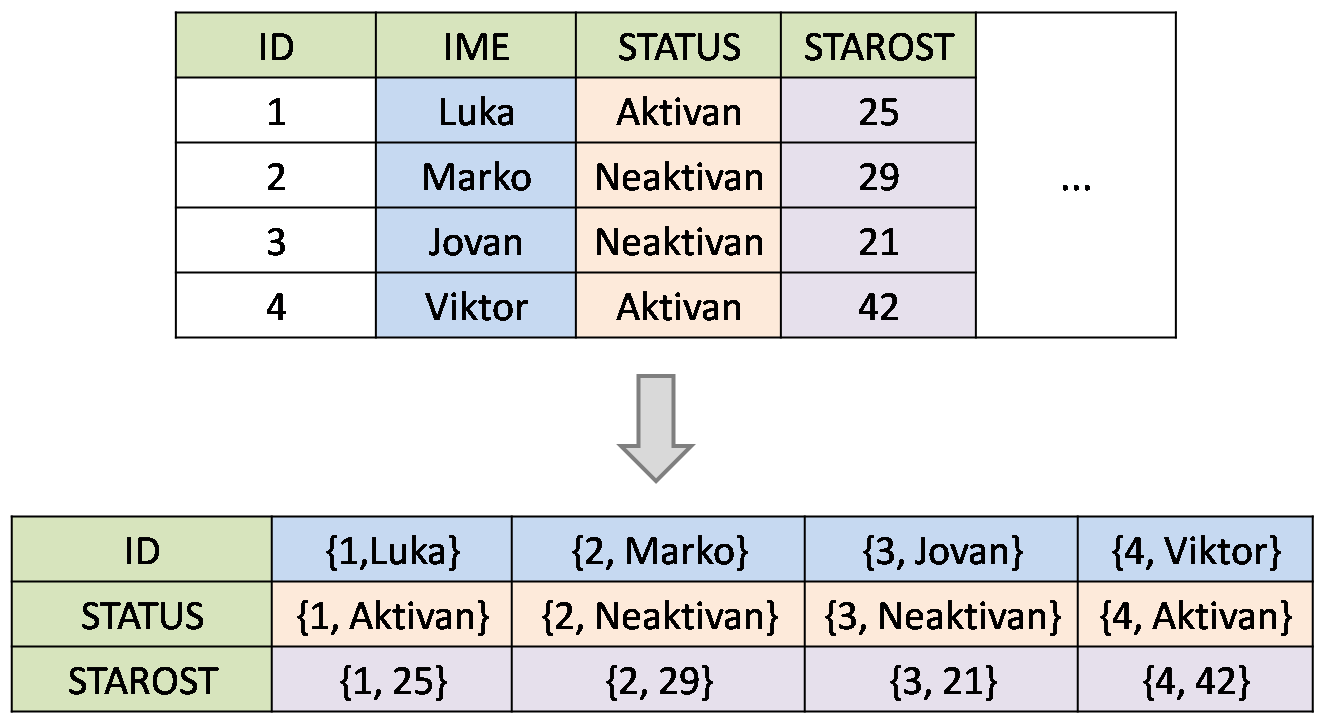
\includegraphics[width=0.9\textwidth]{relational-column-oriented.png}
  \caption{Kolonski orijentisan format}
  \label{fig:grafikon}
\end{figure}

\subsection{Popularni algoritmi kompresije kolonski orijentisanog modela}

Neke od najpoznatijih algoritama kompresije koje kolonski orijentisan model koristi i koji će biti opisani u nastavku jesu: enkodiranje zasnovano na rečniku, enkodiranje po broju ponavljanja i delta enkoding \cite{ColumnarOptimizations}\footnote{Važno je napomenuti da relacioni modeli imaju svoje mehanizme kompresije podataka koji u ovom radu nisu analizirani.}.

Enkodiranje zasnovano na rečniku (engl. \textit{Dictionary based encoding}), slika 2.2., funkcioniše tako što se napravi mapa vrednosti koja sadrži svaku vrednost kolone koja je prisutna među podacima. Kao vrednost kolone tada se ne upisuje konkretna vrednost, već ključ iz rečnika koji je mapiran na tu vrednost. Veličina ključa je srazmerna veličini mape, te je ovaj vid kompresije najpogodniji za kolone koje imaju mali broj vrednosti koje se ponavljaju.

\begin{figure}[!ht]
  \centering
  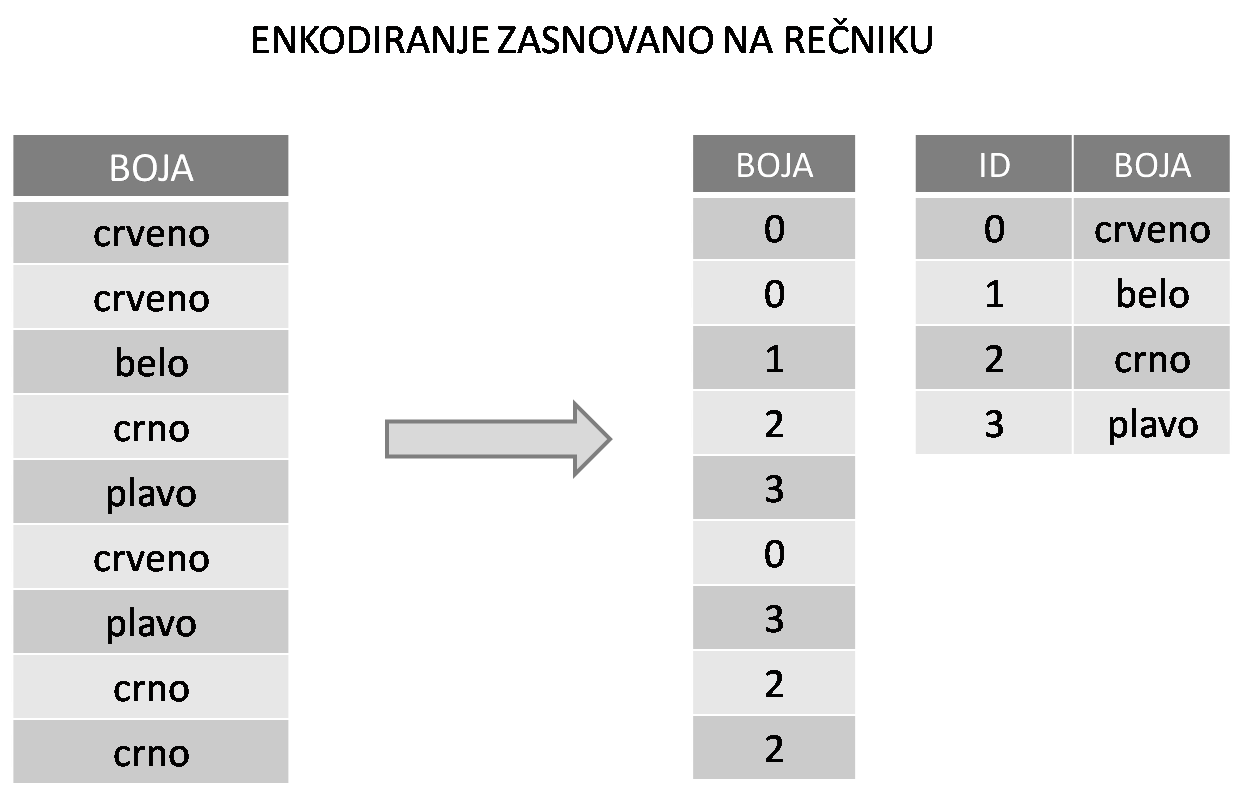
\includegraphics[width=0.7\textwidth]{DictionaryEncoding.png}
  \caption{Enkodiranje zasnovano na rečniku}
  \label{fig:grafikon}
\end{figure}


Enkodiranje po broju ponavljanja  (engl. \textit{Run Length Encoding}) , slika 2.3., funkcioniše tako što se uz svaku vrednost koja se ponavlja čuva i broj ponavljanja te vrednosti. Na taj način se izbegava pojava duplikata na uzastopnim adresama u memoriji. Ovaj vid kompresije najpogodniji je za kolone koje su sortirane i imaju ponavljajuće vrednosti.

\begin{figure}[!ht]
  \centering
  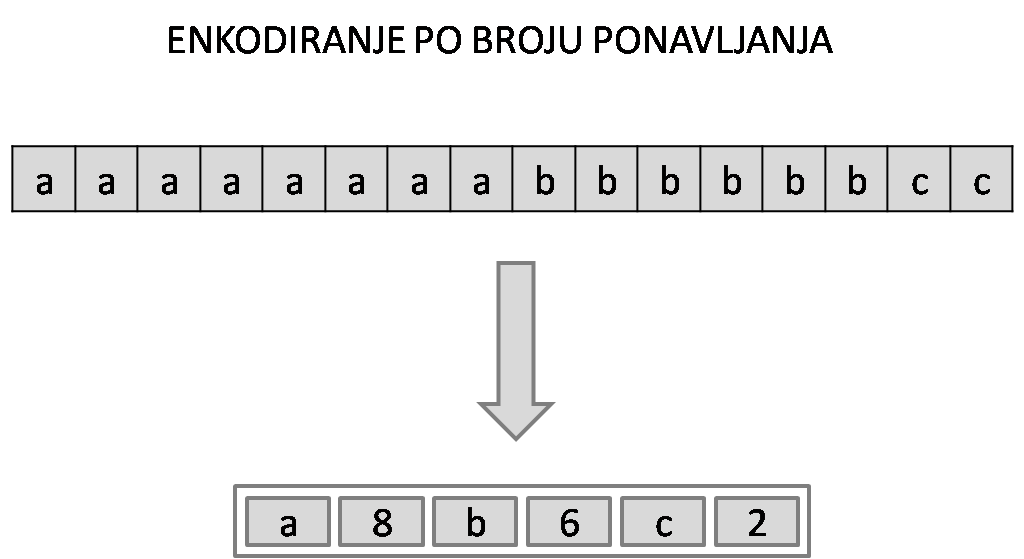
\includegraphics[width=0.7\textwidth]{run-length-encoding.png}
  \caption{Enkodiranje po broju ponavljanja}
  \label{fig:grafikon}
\end{figure}


Delta enkodiranje algoritam kompresije, slika 2.4. funkcioniše tako što se u kolonama ne čuvaju same vrednosti već razlike između uzastopnih vrednosti. Očigledan primer primene ove kompresije je datumska kolona. U tom slučaju  je dovoljno da izaberemo neki referentni datum i da za ostale vrednosti čuvamo razliku u odnosu na njega.

\begin{figure}[!ht]
  \centering
  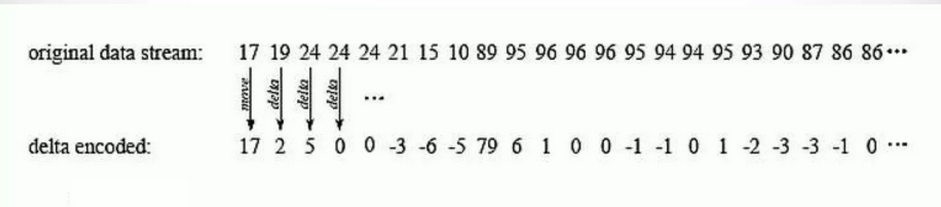
\includegraphics[width=1\textwidth]{delta-encoding.png}
  \caption{Delta enkodiranje}
  \label{fig:grafikon}
\end{figure}

\subsection{HBase}

HBase je kolonski orijentisana nerelaciona baza podataka nastala 2007. godine kao prototip \textit{BigTable} baze koja je modelovana u okviru Google-ovog članka iz 2006.godine\cite{BigTable}. 

Model podataka koji HBase koristi podrazumeva da se svaka tabela sastoji iz familije kolona, a da svaka familija kolona sadrži određeni skup kolona.  S obzirom da će se kolone koje pripadaju jednoj familiji sladištiti blizu na disku, cilj je da atributi, odnosno kolone koje su po prirodi slične, pripadaju istoj familiji kolona, kako bi se nad njima mogli primeniti algoritmi kompresije. HBase nudi fleksibilnost strukture podataka, što znači da, da bismo neki podatak skladištili ne moramo unapred da definišemo skup kolona koji pripada nekoj tabeli , ali moramo definisati skup familija kolona te tabele.

Redovi u HBase-u, odnosno njihovi ključevi sortirani su rastuće, tako da se za pretragu po ključu koristi binarna pretraga. Ovo svojstvo daje na važnosti dizajniranju ključa jer je poželjno da svako čitanje podataka ide po ključu ili njegovom prefiksu \cite{hbaseSchema}. 

Vrednosnu ćeliju u HBase tabeli određuje ključ reda, ime kolone te vrednosne ćelije, kao i familija kojoj kolona pripada, slika 2.5.

HBase nije ACID baza podataka, ali nudi sledeće garancije \cite{hbaseACID}: 

\begin{enumerate}
\item[\textbullet] Atomičnost pri radu sa jednim redom tabele koja se ogleda u tome što će svaka izmena reda u potpunosti uspeti, ili u potpunosti propasti.
\item[\textbullet] Svako čitanje reda iz tabele vratiće stanje reda koje je bilo aktuelno najranije u trenutku kada je čitanje započeto. 
\end{enumerate}

\begin{figure}[!ht]
  \centering
  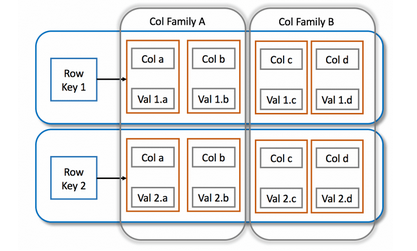
\includegraphics[width=0.8\textwidth]{colFamily.png}
  \caption{HBase model}
  \label{fig:grafikon}
\end{figure}

HBase podatke može čuvati na lokalnom fajl sistemu ili na \textit{Hadoop} distruiranom fajl sistemu(HDFS). HDFS je distribuiran fajl sistem koji ima visok prag tolerancije na greške (\textit{fault tolerance}). HDFS klaster sastoji se iz HDFS master čvorova (\textit{Namenode}) i HDFS čvorova sa podacima (\textit{DataNode}). HDFS master čvor radi sa metainformacijama samog fajl sistema, kao što su izmena direktorijuma, brisanje direktorijuma i sl. Fajlovi na HDFS su interno podeljeni na blokove, gde se svaki od blokova može replikovati i skladištiti na bilo kom od HDFS čvorova sa podacima. O mapiranju blokova fajlova na HDFS čvorove sa podacima brine HDFS master čvor. HDFS čvorovi sa podacima odgovorni su za izvršavanje operacija čitanja i pisanja fajlova na zahtev klijenata. Pored toga HDFS čvorovi sa podacima mogu kreirati, brisati blokove a i replikovati ih, u skladu sa instrukcijama HDFS master čvora \cite{hdfs}.

Arhitektura HBase klastera sastoji se iz tri glavne komponente: master server, region server i \textit{zookeeper}.

Master server  je komponenta HBase klastera koja se bavi metainformacijama tabela HBase-a. Pored toga, on region serverima dodeljuje regione i bavi se balansiranjem opterećenja klastera (\textit{load balancing}).

Region server zadužen je za rad sa dodeljenim regionima od strane master servera. Region je skup redova HBase-a u nekom rasponu ključeva. Kako bi region server mogao da piše i čita podatke regiona, on održava WAL (engl \textit{Write Ahead Log}) fajl, MemStore fajl kao i HFile fajlove. Svaka izmena, pre nego što je sačuvana na disku, upisuje se u vidu loga (\textit{commit log}) u WAL, tako da u slučaju pada sistema pre nego što su se izmene sačuvale, logovi koji se nalaze u WAL fajlu mogu rekonstruisati stanje pre pada sistema \cite{wal}. MemStore je fajl u koji se upisuju podaci pre nego što se sačuvaju na disku. On predstavlja vid bafera koji kada se popuni, reflektuje podatke na disk, odnosno na HFile. HFile fajl sadrži konkretne podatke u predviđenom formatu. Oni se mogu skladištiti na lokalnom fajl sistemu ili na HDFS, u zavisnosti od konfiguracije.

Zookeeper predstavlja most u komunkaciji komponenti HBase klastera \cite{zookeeper}. Zookeeper servis  sinronizuje sve master i region servere, ima evidenciju o tome koji je master server aktivan a koji pasivan, koji region serveri više nije dostupni itd.

HBase dozvoljava dva režima: samostalan i distribuirani režim.

U samostalnom režimu HFile fajlovi se mogu čuvati na lokalnom fajl sistemu i korišćenje HDFS-a je opciono, slika 2.6  \footnote{Izvor: https://devstacks.wordpress.com/2017/07/19/apache-hbase-architecture-and-overview}.

Sa druge strane u distribuiranom režimu neophodno je korišćenje HDFS-a za skladištenje, slika 2.7 \footnote{Izvor: https://devstacks.wordpress.com/2017/07/19/apache-hbase-architecture-and-overview}. 

\begin{figure}[!ht]
  \centering
  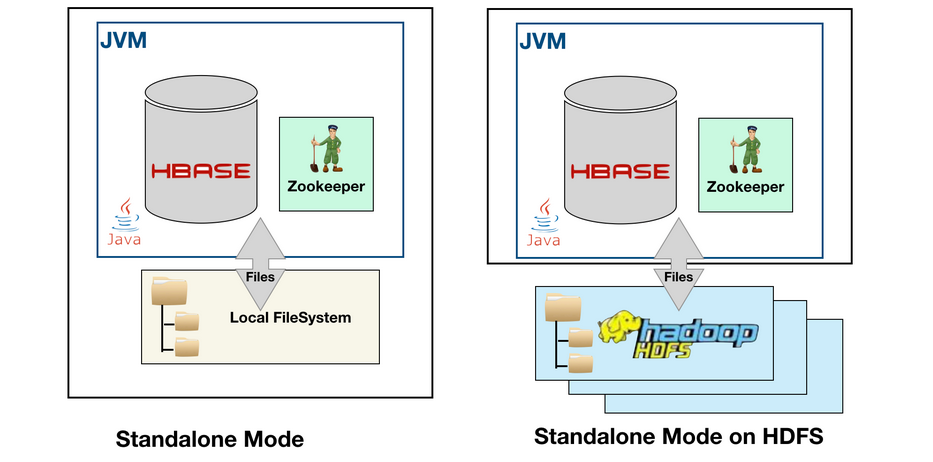
\includegraphics[width=0.9\textwidth]{hbase-standalone.png}
  \caption{HBase - samostalan režim }
  \label{fig:grafikon}
\end{figure}

\begin{figure}[!ht]
  \centering
  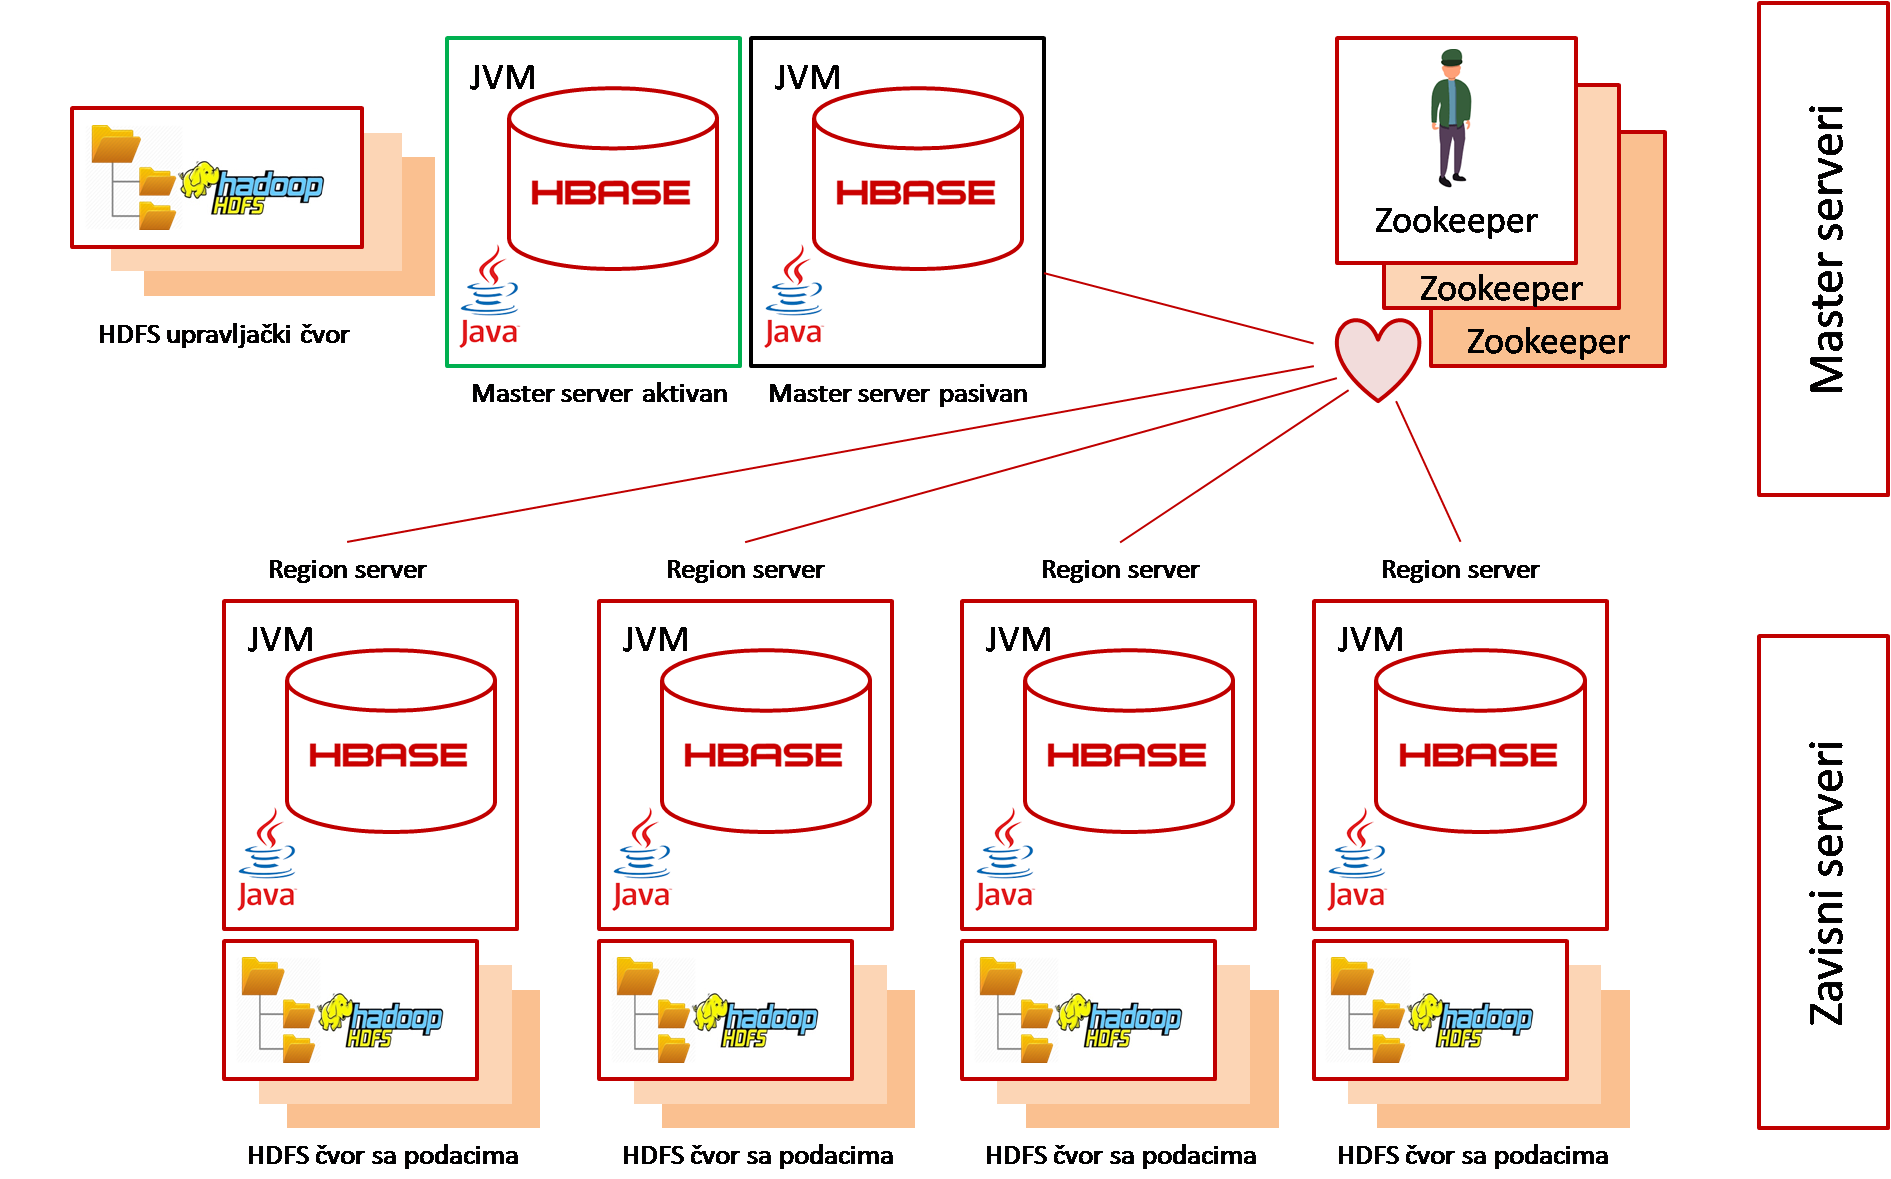
\includegraphics[width=1\textwidth]{hbase-distributed.png}
  \caption{HBase -distribuirani režim}
  \label{fig:grafikon}
\end{figure}


\pagebreak

\section{Glavne razlike između relacionog i kolonski-orijentisanog modela}


\subsection{Normalizacija i denormalizacija}

U relacionim modelima često se radi na izbegavanju \textit{redudantnosti} u podacima. Redudantni podaci zauzimaju višak prostora na disku i otežavaju kasnije održavanje sistema. Kako bi se izbegla redudantnost, postoje postupci koji nam pomažu da organizujemo podatke tako da redudantnost umanjimo. Proces izmene logičkog modela baze podataka u cilju oslobađanja od redundantosti podataka naziva se normalizacija. U zavisnosti od toga koja pravila zadovoljava određena relacija, dodeljuje joj se odgovarajuća normalna forma. Neke od normalnih formi relacionog modela su: 1. normalna forma, 2. normalna forma, 3. normalna froma, normalna forma elementarnog ključa, Bojs-Kodova normalna forma, 4. normalna forma, normalna forma esencijalnih torki, normalna forma bez redundansi, normalna forma superključeva, 5. normalna forma, normalna forma domena i ključa.

Normalizovani modeli obično raspolažu velikim brojem stranih ključeva što dovodi do povećanja broja tabela kojima se pristupa u upitima, a time i povećanja broja operacija čitanja sa diska, što može uticati na performanse.

Denormalizacija je strategija koja se koristi kod modela kod kojih je neophodno ubrzati operacije čitanja podataka, odnosno umanjiti broj tabela kojima je neophodno pristupiti kako bi se neki skup podataka pročitao iz baze podataka, po cenu uvećanja memorijskog zauzeća. Kako kolonski orijentisane baze podataka često rade na infrastrukturama koje su horizontalno skalabilne, uvećanje memorijskog zauzeća, kako bi se ubrzao pristup podacima, jeste cena koju su spremne da plate.
 
Neke od tehnika denormalizacije su:  spajanje kolone, horizontalna podela tabele, vertikalna podela tabele i uvođenje izvedene kolone. 

Spajanje kolone, slika 2.8. je dodavanje kolone kojoj bi se često pristupalo preko stranog ključa.

\begin{figure}[!ht]
  \centering
  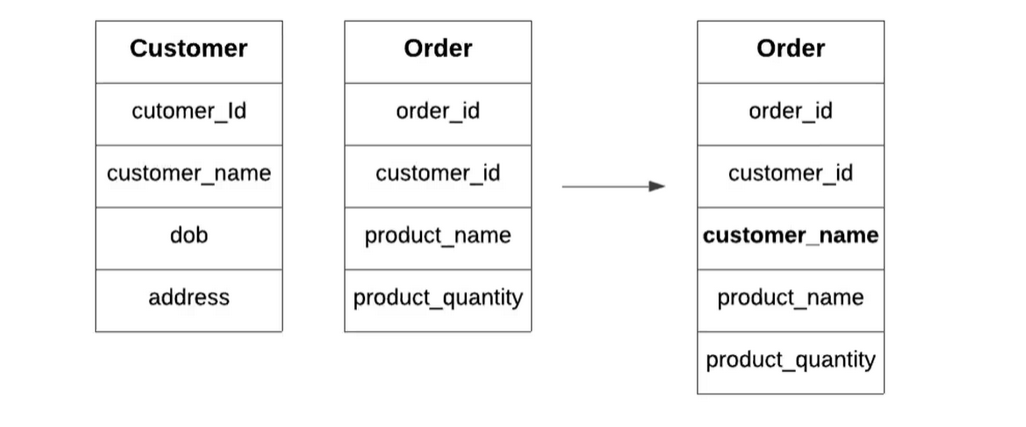
\includegraphics[width=0.7\textwidth]{denormalizacija.png}
  \caption{Spajanje kolone}
  \label{fig:grafikon}
\end{figure}

Horizontalno deljenje tabele, slika 2.9. podrazumeva da se na osnovu prirode podataka jedna tabela podeli na više tabela tako da se čitanje svede samo na čitanje grupe redova. 

\begin{figure}[!ht]
  \centering
  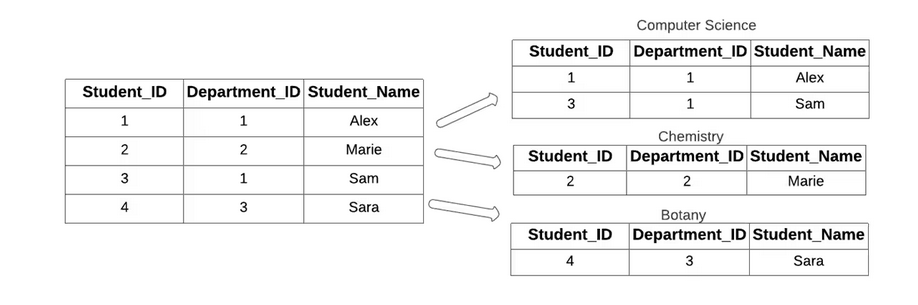
\includegraphics[width=0.9\textwidth]{denormalizacija2.png}
  \caption{Horizontalna podela tabele}
  \label{fig:grafikon}
\end{figure}

Vertikalno deljenje tabele, slika 2.10. podrazumeva da se tabela podeli grupisanjem kolona koje se često čitaju zajedno. 

\begin{figure}[!ht]
  \centering
  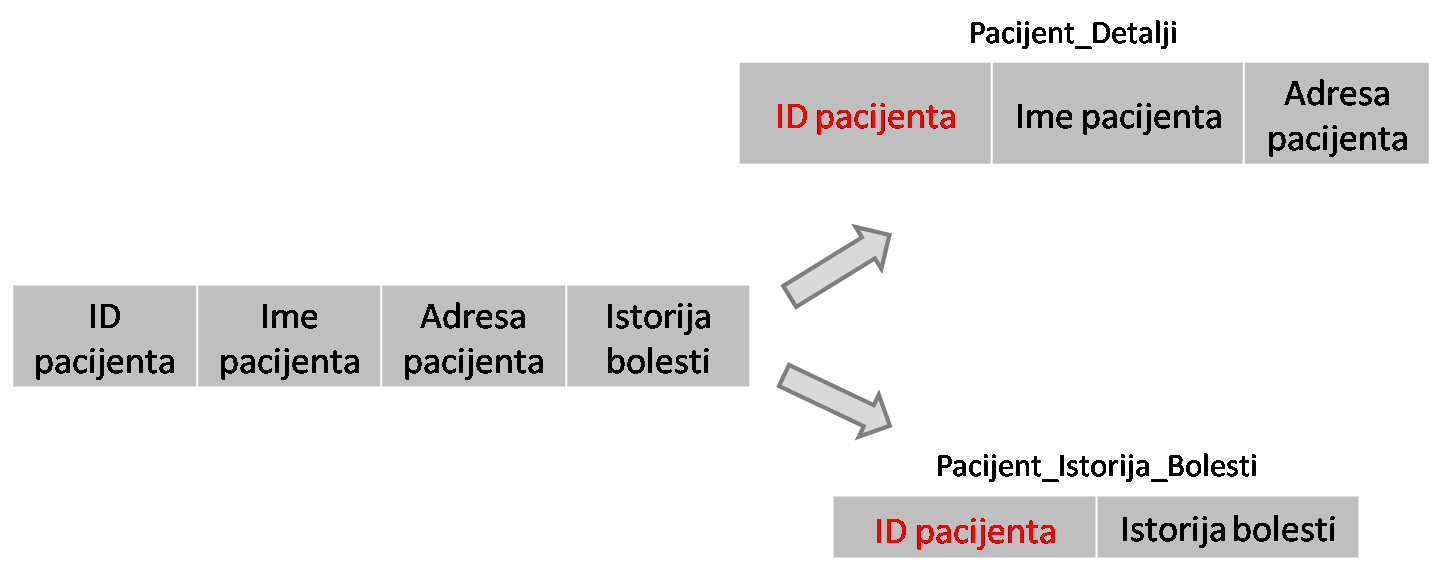
\includegraphics[width=0.9\textwidth]{denormalizacija3.png}
  \caption{Vertikalna podela tabele}
  \label{fig:grafikon}
\end{figure}

Uvođenje izvedene kolone, slika 2.11. predstavlja dodavanje kolone koja čuva rezultat neke agregatne funkcije. Time se izbegava da se pri svakom čitanju ta agregatna funkcija izvršava, već se pri ažuriranju stanja ta vrednost ažurira, da bi se rezultat kasnije mogao samo pročitati.


\begin{figure}[!ht]
  \centering
  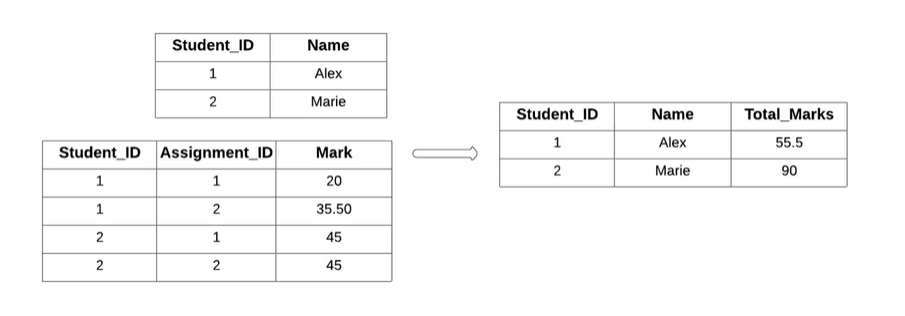
\includegraphics[width=0.9\textwidth]{denormalizacija4.png}
  \caption{Uvođenje izvedene kolone}
  \label{fig:grafikon}
\end{figure}
\pagebreak

\subsection{ACID i BASE}

Transakcija je logička jedinica posla pri radu sa podacima \cite{URBP}. Kod relacionih modela jednu transakciju karakteriše: atomičnost, konzistentost, izolovanost i trajnost (ACID).

Atomičnost transakcije se može objasniti pravilom: Jedna transakcija se izvršava u celini ili se ne izvršava nijedan njen deo, odnosno dejstvo transakcije je nedeljivo. 

Konzistentost transakcije znači da dejstvo transakcije ne može ostaviti stanje koje narušava integritet baze podataka.

Izolovanost transakcije čini da transakcije ne mogu uticati međusobno jedna na drugu, odnosno, kada se jedna transakcija pokrene, pa sve dok se ne završi, za nju, izmena neke druge transakcije neće biti vidljiva.

Trajnost transakcije garantuje da će kompletirana transakcija u slučaju prekida rada sistema pre nego što su izmene upisane na disk, biti upamćena i izvršena nakon restarta sistema. Svaka izmena se upisuje u log fajl pre nego što je upisana na disk, kako bi se operacije mogle poništiti u slučaju poništavanja transakcije.

Ova svojstva obično karakterišu transakcije u relacionom modelu, kada konzistentost baze ima veći prioritet od brzine i dostupnosti. Kod kolonski orijentisanih baza podataka, posebno u distribuiranom režimu, dostupnost i brzina često imaju veći prioritet od stalne konzistentosti. Kod njih se koristi alternativni pristup karakterizacije transakcije - BASE. BASE transakcije zadovoljavaju sledeća svojstva: suštinska raspoloživost, postojanje mekog stanja i konvergentna konzistentnost.

Suštinska raspoloživost omogućava maksimalnu dostupnost čitanja i pisanja, ali bez garancije konzistentosti.

Meko stanje daje mogućnost da se stanje baze podataka menja čak i kada nijedna transakcija nije u toku, i to u periodu postizanja konzistetnosti.

Konvergentna konzistentnost obezbeđuje da će baza podataka u slučaju da nema novih upisa, postati konzistentna kroz neki vremenski period. 

\subsubsection{Distribuiranost i CAP teorema}

Kako bi se postigla skalabilnost, umanjilo kašnjenje odgovora (engl \textit{latency}) i povećala dostupnost sistema u slučaju nepredviđenih okolnosti, podaci često bivaju distribuirani na više međusobno povezanih jedinica. Takve baze podataka nazivamo distribuiranim.
Dva načina distribuiranja podataka su: fragmentacija i replikacija \cite{URBP}. 

Fragmentacija distribuira podatke tako što se veliki skupovi podataka podele na fragmente i čuvaju na različitim čvorovima. Fragmentacija može biti horizontalna, vertikalna ili mešovita. Horizontalna fragmentacija (particionisanje) predstavlja podelu skupa redova tabele na podskupove po određenom kriterujmu. Vertikalna fragmentacija predstavlja podelu skupa kolona na podskupove po određenom kriterijumu.  Mešovita fragmentacija predstavlja kombinaciju horizontalne i vertikalne fragmentacije.

Replikacija podrazumeva da se više kopija podataka čuva na različitim čvorovima, odnosno replikama. Broj replika svakog od podataka predstavlja faktor replikacije. Ukoliko neki od čvorova postane nedostupan, klijentski zahtevi mogu biti obrađeni na nekom od preostalih čvorova. To sisteme koji koriste replikaciju čini pouzdanijim. Kako bi svaka replika bila ažurna neophodno je da se svaka izmena podataka propagira do svakog čvora. Najpoznatiji model po kojem se to realizuje je \textit{master-slave} (\textit{ROWA - Read one write all}). Postoje i alternative: kao što su \textit{multimaster}, konsenzus kvoruma itd. U \textit{master-slave} modelu jedna od replika izabrana je da bude master replika i svaka izmena podataka mora ići kroz nju. Dalje, ona izmene propagira do ostalih zavisnih (\textit{slave}) replika. Čitanje podataka se sa druge strane, može 
raditi sa bilo kog čvora što omogućava brži pristup podacima, Slika 2.12.

\begin{figure}[!ht]
  \centering
  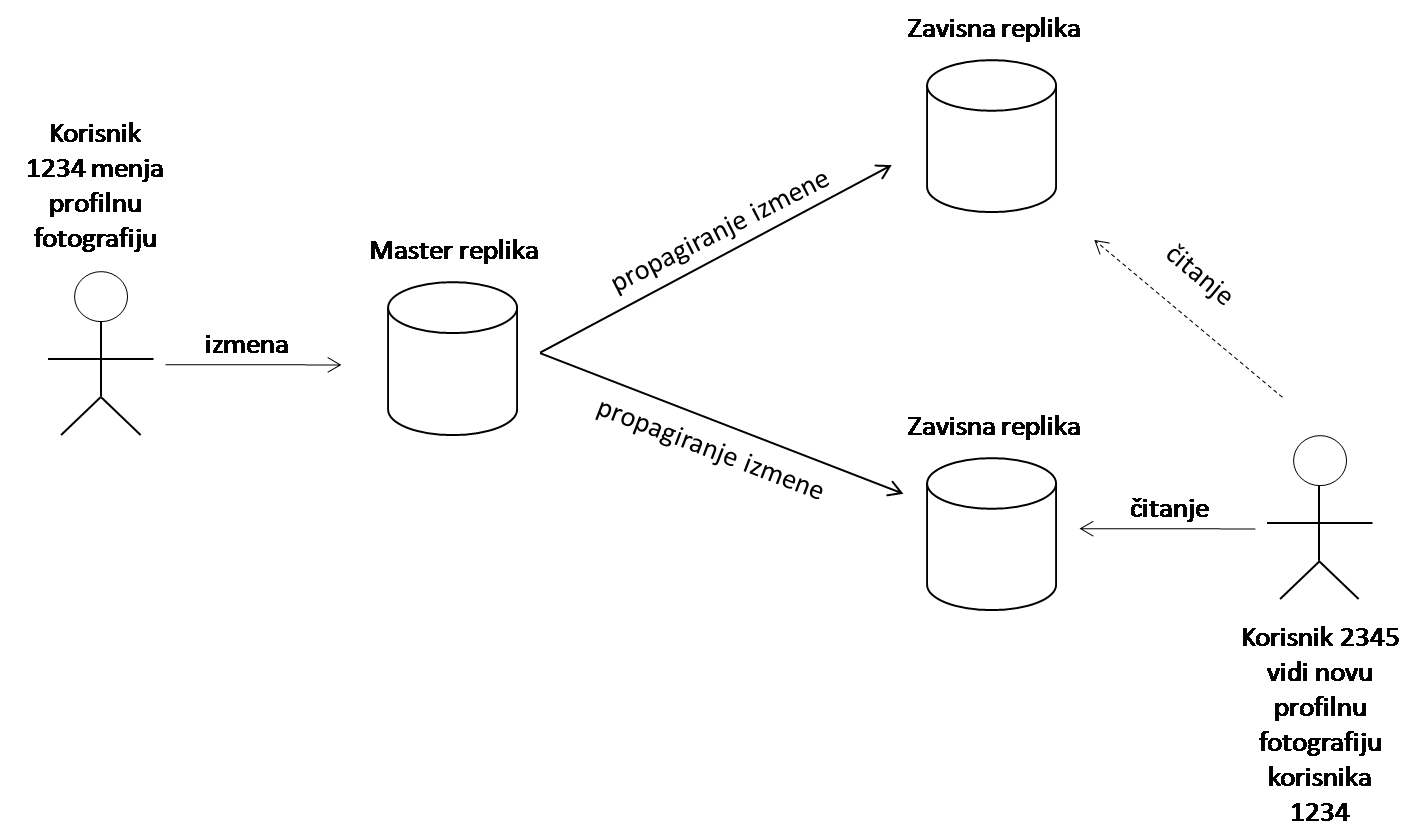
\includegraphics[width=0.8\textwidth]{master-slave.png}
  \caption{Master-slave replikacija}
  \label{fig:grafikon}
\end{figure}


Replikacija može biti sinhrona i asinhrona. Kod sinhrone replikacije kada izmena dođe do master čvora, on pre nego što klijentu vrati odgovor da je izmena uspešno sačuvana, sačeka da mu svaki zavisni čvor potvrdi da je izmena uspešno upisana kod njega. Sinhrona replikacija je karakteristična za sisteme koji garantuju da će klijent pri čitanju podatka sa bilo koje replike imati ažurno stanje, međutim, cena toga je sporije ažuriranje podataka, kao i umanjena dostupnost, s obzirom da ukoliko neki od zavisnih čvorova postane nedostupan, on ne može master čvoru potvrditi da je izmena upisana na njega, pa samim tim ni master ne može klijentu potvrditi da je izmena uspešno upisana. Kod asinhrone replikacije, kada izmena podataka dođe do mastera i on tu izmenu propagira ka ostalim zavisnim čvorovima, master ne čeka odgovor od zavisnih čvorova, već ukoliko je izmena uspešno upisana na njega on klijentu vraća potvrdu o sačuvanoj izmeni. Asinhrona replikacija obično nudi bolje performanse i veću dostupnost servisa, po cenu toga da čitanje sa neke od replika može vraćati zastarele podatke.


\pagebreak
Replikacija i fragmentacija se obično primenjuju zajedno, tako što se podaci prvo podele na particije, a svaka particija replikuje na više čvorova \cite{ColumnarOriented}, slika 2.13. 

\begin{figure}[!ht]
  \centering
  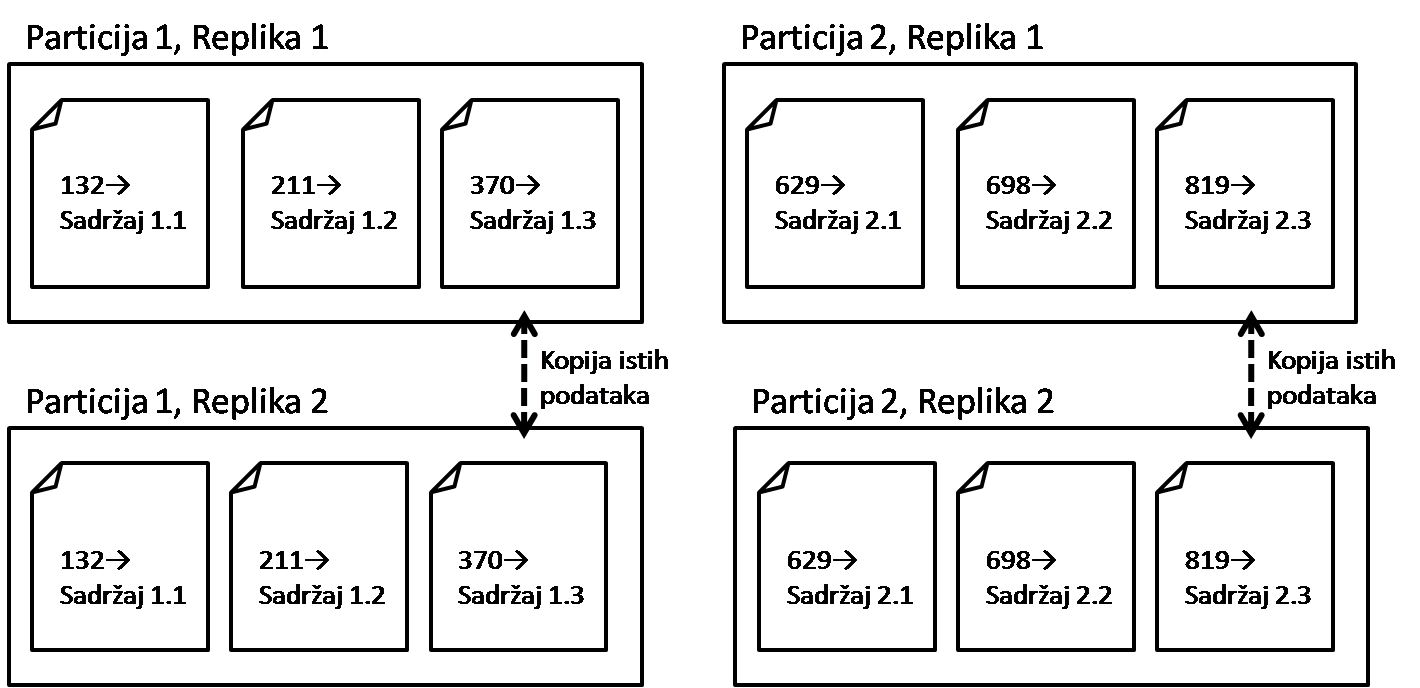
\includegraphics[width=0.9\textwidth]{replica-partition.png}
  \caption{Replikacija i fragmentacija}
  \label{fig:grafikon}
\end{figure}

Kvalitet distribuiranih baza podataka ogleda se kroz tri svojstva: konzistentost, raspoloživost i tolerancija razdvojenosti.

Konzistenost u ovom kontekstu razlikuje se od konzistentosti transakcije. U kontekstu distribuiranih sistema, konzistetnost je svojstvo baze podataka, koje garantuje da će odgovor koji se šalje sa bilo kog čvora klastera (ukoliko odgovora ima) biti ažuran. Na ovom svojstvu obično insistiraju sistemi koji u distribuiranom okruženju koriste sinhronu replikaciju.

Raspoloživost je svojstvo koje obezbeđuje da će baza uvek vratiti nekakav odgovor. Na ovom svojstvu insisitiraju sistemi koji u distribuiranom okruženju koriste asinhronu replikaciju.

Tolerancija razdvojenosti znači da će u slučaju delimičniih otkaza unutar klastera, sistem i dalje funkcionisati.

CAP teorema koju je formulisao Eric Brewer \footnote{Eric Allen Brewer profesor računarskih nauka na Univerzitetu Kalifornija, Berkli}, navodi da distribuirana baza podatka ne može istovremeno ispunjavati sva tri svojstva, slika 2.12.

Obzirom da je konzistentost i dostupnost u praksi skoro nemoguće dostići, distribuirane baze podataka organizuju se u skladu sa tim da li se veći prioritet daje dostupnosti ili stalnoj konzistentosti. Priroda baza podataka koji koriste relacioni model obično je takva da daju prioritet konzistetnosti, pa se od njih očekuje da u distribuiranom okruženju osim konzistetnosti nude i toleranciju razdvojenosti, za razliku od kolonski orijentisane nerelacione baze koja konzistetnost ne garantuje (garantuje konvergentnu konzistenciju), ali uz toleranciju razdvojenosti nudi stalnu dostupnost.

\begin{figure}[!ht]
  \centering
  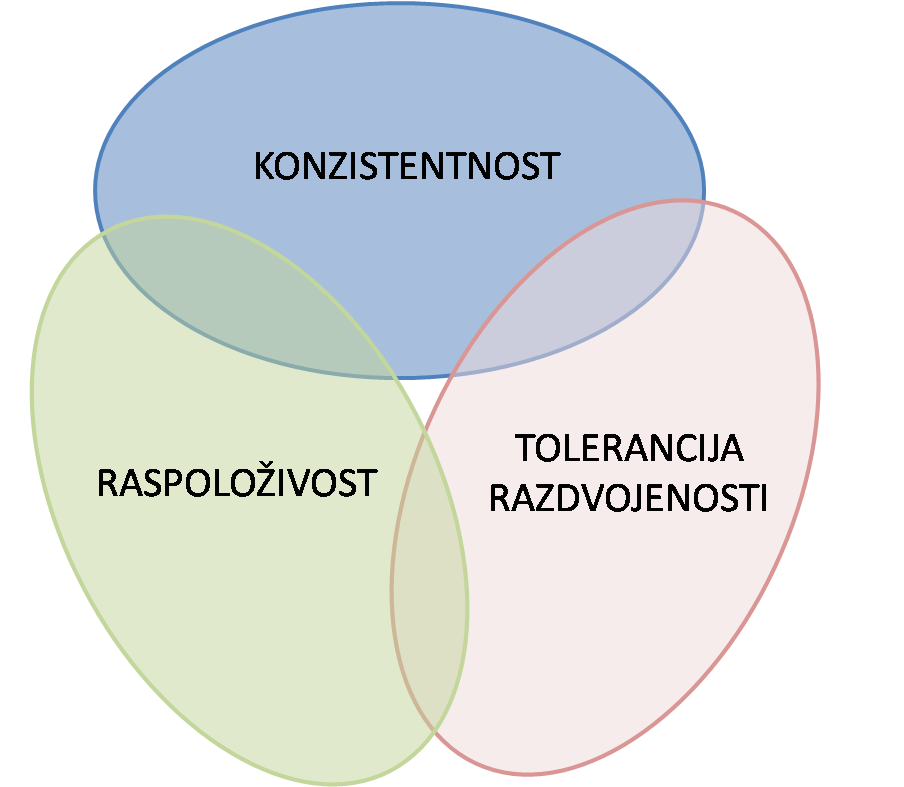
\includegraphics[width=0.6\textwidth]{cap.png}
  \caption{CAP teorema}
  \label{fig:grafikon}
\end{figure}

\chapter{Slučajevi upotrebe}

Kako bi se postigao dovoljan dokaz koncepta (engl. \textit{proof of concept}) kreirano je više scenarija koji na različit način pristupaju radu sa podacima. Scenariji, odnosno slučajevi upotrebe koji su testirani u ovom radu jesu: 
\begin{enumerate}
\item Onlajn transakciono procesiranje (OLTP)
\item Onlajn analitičko procesiranje (OLAP)
\item Distribuirano okruženje
\end{enumerate}


\section{Onlajn transakciono procesiranje (OLTP)}
Onlajn transakciono procesiranje predstavlja procesiranje podataka koje se sastoji iz velikog broja transakcija.  Svaka pojedinačna transakcija obično deluje na manjem skupu podataka i obično uključuje njihovu izmenu, a kada se radi čitanje podataka, ono je obično po ključu \cite{oltp}. Kod ovakvog vida procesiranja, gde su izmene podataka česte, čuvanje integriteta podataka prilikom tih upisa je prioritet, pa je OLTP često sastavni deo finanskijskih sistema, sistema za rezervacije i sl.
Konkretan scenario koji će u radu simulirati OLTP okruženje je prebacivanje sredstava sa jednog računa na drugi. Svako prebacivanje novca predstavljaće jednu poslovnu transakciju koja se sastoji iz više transakcija baze podataka. Definicija poslovne transakcije koja se koristi za testiranje delom je preuzeta iz TPC-C specifikacije \cite{tpcc}. 

Jedna poslovna transakcija sastoji se iz tri transakcije baze podataka: kreiranje transfera sredstava (\textit{createFXTransaction}), izvršavanje uplate (\textit{executePayment}) i provera statusa transfera (\textit{checkTransactionStatus}).

CreateFXTransaction sastoji se iz provere sredstava na računu korisnika i unosa novog transfera u tabelu.

ExecutePayment radi ažuriranje računa korisnika i menja status transfera

CheckTransaction dohvata status transfera.

\section{Onlajn analitičko procesiranje (OLAP)}

Onlajn analitičko procesiranje sačinjeno je od velikog broja čitanja podataka i manjeg broja izmena podataka (koje su obično masivne - \textit{bulk}). Upiti koji se koriste obično imaju parametre, visok nivo kompleksnosti i visok procenat podataka kojima pristupaju. OLAP je obično sastavni deo sistema koji nude podršku za donošenje poslovnih odluka, generisanje složenih izveštaja kao i bilo koji vid korišćenja velike količine podataka koristeći složene upite i operacije. Scenario koji se simulira u ovom radu u svrhu testiranja, jeste primer funkcionisanja trgovinskog lanca sa skupom svojih mušterija, proizvoda, dobavljača i narudžbina. Korišćen model delom je preuzet iz TPC-H specifikacije \cite{tpch}. Test će se sastojati iz paralelnog izvršavanja složenog upita koji iz tabele sa stavkama narudžbina izvlači vrednosti agregatnih funkcija određenih kolona grupisanih po statusu. Parametri upita su dan slanja narudžbine i status po kojima filtriramo rezultat.


\section{Distribuirano okruženje}

U svrhu demonstracije i merenja performansi HBase-a u distribuiranom okruženju biće iskoršćeni testovi iz testiranja OLTP i OLAP  scenarija. S obzirom na to da se testiranje izvršava na jednom računaru, koristiće se HBase klaster sa jednim region serverom, jednim master serverom, zookeeper servisom,  jednim HDFS čvorom podataka i jednim HDFS master čvorom. Svi oni će se izvršavati kao zasebni procesi. Usled složenosti implementacije distribuiranog relacionog sistema (u ovom slučaju PostgreSQL-a), za distribuirano okruženje primer je dat samo za HBase.


\chapter{Merenje performansi po modelima}

\section{Opis platforme za testiranje}

Za predstavnike baza podataka izabrani su HBase (kao predstavnik kolonski orijentisane nerelacione baze podataka) i PostgreSQL (kao predstavnik relacione baze podataka)\footnote{Napomena: Kako su za predstavnike izabrani PostgresSQL i HBase, rezultati dobijeni u nastavku su rezultati poređenja konkretnih predstavnika, i nisu opšti za sve relacione i kolonski orijenisane nerelacione baze podataka.}.  Kao okruženje za izvršavanje testova  korišćen je \textit{docker}. Serveri oba predstavnika biće pokrenuti kao nezavisni kontejneri, slika 4.1. 

\begin{figure}[!ht]
  \centering
  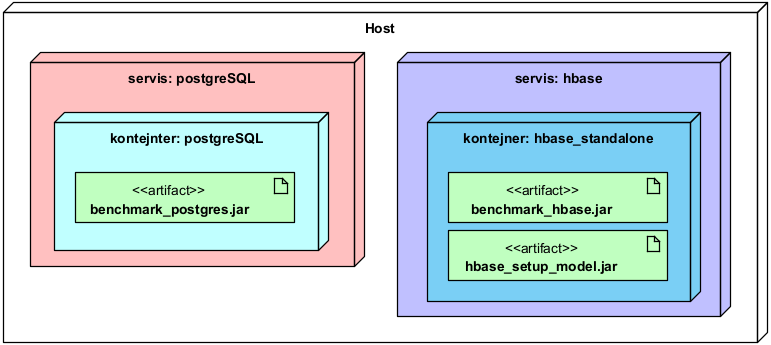
\includegraphics[width=0.9\textwidth]{deployment_diagram.png}
  \caption{Platforma testiranja}
  \label{fig:grafikon}
\end{figure}


\section{Merenje performansi u OLTP okruženju}

Model baze podataka za testiranje u OLTP okruženju koji se koristu u radu, sastoji se iz četiri tabele:


\begin{enumerate}
\item[\textbullet] \textbf{fxrates}: {
	Sadrži informacije o kursu valutnih parova. Sadrži 16 redova.
}
\item[\textbullet] \textbf{fxuser}:{
	Podaci o korisnicima. Sadrži  \numprint{30000} redova.
}
\item[\textbullet] \textbf{fxaccount}:{
	Podaci o računima korisnika. Sadrži  \numprint{120000} redova.
}
\item[\textbullet] \textbf{fxtransaction}:{
	Sadrži informacije o transferima, odnosno transakcijama sredstava.
}
\end{enumerate}


\lstset{
  language=sql,
  captionpos=bottom,
  basicstyle=\footnotesize\ttfamily,
  keywordstyle=\color{black},
  backgroundcolor = \color{LemonChiffon1},
  numbers=left,
  showstringspaces=false,
  frame=single
}

\begin{lstlisting}[title={setup-postgres-model.sql - Kreiranje PostgreSQL modela},captionpos=b]

create table postgresdb.fxrates (
	currency_from  varchar(50) not null,
	currency_to varchar(50) not null,
	rate real not null,
	primary key(currency_from,currency_to)
);

create table postgresdb.fxuser (
	id  integer primary key,
	username varchar (50) unique not null,
	password varchar (50) not null,
	start_balancecurrency varchar (10) not null,
	start_balance real not null,
	firstname varchar(100) not null,
	lastname varchar(100) not null,
	street varchar(100) not null,
	city varchar(100) not null,
	state varchar(100) not null,
	zip varchar(50) not null,
	phone varchar(30) not null,
	mobile varchar(30) not null,
	email varchar(50) unique not null,
	created timestamp not null
);

create table postgresdb.fxaccount (
	id  integer primary key,
	fxuser integer not null  references postgresdb.fxuser(id),
	currency_code varchar(10) not null,
	balance real not null,
	created timestamp not null,
	unique (fxuser, currency_code)
);

create table postgresdb.fxtransaction (
	id integer primary key,
	fxaccount_from  integer references postgresdb.fxaccount(id),
	fxaccount_to  integer references postgresdb.fxaccount(id),
	amount numeric(15,2) not null,
	status varchar(50) not null,
	entry_date timestamp not null
);

\end{lstlisting}

\begin{lstlisting}[title={setup-hbase-model.sh - Kreiranje HBase modela},captionpos=b]
create fxrates, 'data';
create fxuser, 'data';
create fxaccount, 'data';
create fxtransaction, 'data';
\end{lstlisting}

Kao što je ranije spomenuto, poslovna transakcija koja se testira jeste prebacivanje sredstava sa jednog računa na drugi.  Ona se sastoji iz tri dela: kreiranje transfera sredstava (\textit{createFxTransaction}), izvršavanja uplate(\textit{executePayment}) i provera 
statusa transfera (\textit{checkTransactionStatus}).

CreateFXTransaction prvo pročita stanje naloga sa kojeg treba preneti sredstva, nakon toga čita kurs odgovarajućeg valutnog para i ukoliko ima dovoljno sredstava na računu, u tabelu sa transferima upisuje transfer u statusu \textit{NEW}.

\pagebreak

\begin{lstlisting}[title={CreateFXTransaction},captionpos=b]

select fa.balance
from fxaccount fa
where fa.id = ?;

select fr.rate
from fxrates fr
where fr.currency_to = ? and fr.currency_from = ?;

insert into fxtransaction
(id,fxaccount_from, fxaccount_to, amount, status, entry_date)
values(?,?,?,?,?,?);
\end{lstlisting}

ExecutePayment prvo pročita stanja sa naloga koji učestvuju u transferu, menja im balans i nakon toga transferu menja status.

\begin{lstlisting}[title={ExecutePayment},captionpos=b]

select balance
from fxaccount
where id = ?;

update fxaccount
set balance = ?
where id = ?;

select balance
from fxaccount
where id = ?;

update fxaccount
set balance = ?;
where id = ?;

update fxtransaction
set status = ?
where id = ?;

\end{lstlisting}
\pagebreak
CheckTransactionStatus za odgovarajuću transakciju čita status po primarnom ključu.


\begin{lstlisting}[title={CheckTransactionStatus},captionpos=b]
select status
from fxtransaction
where id = ?;
\end{lstlisting}


Test ima podršku za paralelno izvršavanje poslovnih transakcija. Parametri testa su \textbf{broj klijenata} (\textit{numOfClients}) i \textbf{broj poslovnih transakcija koje treba izvršiti} (\textit{totalTransactions}). Oba parametra postavljaju se prilikom pokretanja testa, kroz standardni ulaz. Politika dodeljivanja poslovnih transakcija svakom od klijenata je da se ukupan broj poslovnih transakcija ravnomerno podeli svim klijentima, a eventualni ostatak pri podeli dodeljuje se nekom od njih.

\begin{lstlisting}[title={Implementacija politike podele posla klijentima},captionpos=b]
List<Integer> transClientList = new ArrayList<>();
int transToAssign = totalTransactions;
int transPerClient = transToAssign / numOfClients;

for(int i = 0; i<numOfClients;i++){	
   transClientList.add(transPerClient);
   transToAssign-=transPerClient;
}
if (transToAssign > 0) {
   int transForLast = transPerClientList.get(numOfClients - 1);
   transClientList.set(numOfClients - 1, transForLast + transToAssign);
}

assert numOfClients==transClientList.size();
Thread[] threads = new Thread[numOfClients];
for(int i = 0;i<numOfClients;i++){
   threads[i] = new Thread(
      new BenchmarkSingleClientExecutor(
         i*transClientList.get(i),transClientList.get(i)
         )
      );
 }
\end{lstlisting}


Nakon što se klijentu dodeli skup poslovnih transakcija koje treba da obradi, on krene da izvršava sve tri faze svake poslovne transakcije koja mu je dodeljena. Svaki transfer koji učestvuje u poslovnoj transakciji generisan je na osnovu rednog broja poslovne transakcije koju klijent procesira. To je garancija da se ne može desiti da se isti transfer obrađuje više puta, kao i to da dva klijenta ne mogu obrađivati isti transfer.

\begin{lstlisting}[title={BenchmarkSingleClientExecutor.java - Posao klijenta},captionpos=b]

public class BenchmarkSingleClientExecutor implements Runnable {

private final CountDownLatch endSignal;
private final BenchmarkOLTPUtility oltpUtil;
private final int numOfT;
private final int start;

private final Object connection;

@Override
public void run() {

try {
   for (int i = this.start; i < this.start + this.numOfT; i++) {
     FXTransaction fxTransaction = DataGenerator.seedTransacton(i);
     ExecutePaymentInfo executePaymentInfo = 
         oltpUtil.createFXTransaction(connection);
     oltpUtil.executePayment(executePaymentInfo);
     oltpUtil.checkTransactionStatus(fxT);
    }
    endSignal.countDown();
} catch (Exception e) {
     throw new IllegalStateException(e);
 }
}
}
\end{lstlisting}

Priprema okruženja za testiranje podrazumeva kompilaciju java testova, pokretanje docker kontejnera i prebacivanje kompiliranih testova na odgovarajuće kontejnere. Dodatan korak za HBase jeste da se na HBase kontejneru kreira struktura baze podataka. Skripta u nastavku sadrži sve neophodne komande za pokretanje okruženja.

\pagebreak

\begin{lstlisting}[title={prepare-env.sh - Skripta za pokretanje OLTP okruženja},captionpos=b]
#!/bin/bash
echo 'PREPARING ENVIRONMENT...';

export JAVA_HOME="$JAVA_8";
mvn -f ./hbase_setup_model clean compile assembly:single;
mvn -f ./benchmark_hbase clean compile assembly:single;
export JAVA_HOME="$JAVA_17";
mvn -f ./benchmark_postgres clean compile assembly:single;

docker-compose -f docker-compose.yml up --build -d;
docker exec -it hbase-master-1 sh -c "java -jar hbase_setup_model.jar";
\end{lstlisting}

\begin{lstlisting}[title={docker-compose.yml - Definicija kontejnera za OLTP okruženje},captionpos=b]
services: 
  postgres:
    container_name: postgres
    ports:
      - "5433:5432"
    volumes:
      - ./setup_model.sql:/docker-entrypoint-initdb.d/create_script.sql
      - ./benchmark_postgres.jar:/benchmark_postgres.jar
    environment:
      - POSTGRES_PASSWORD=postgres
      - POSTGRES_USER=postgres
      - POSTGRES_DB=postgresdb
    build:
      context: .
      dockerfile: ./Dockerfile_postgres

  hbase:
    image: bde2020/hbase-standalone:1.0.0-hbase1.2.6
    container_name: hbase
    volumes:
      - hbase_data:/hbase-data
      - hbase_zookeeper_data:/zookeeper-data
      - ./hbase_setup_model.jar:/hbase_setup_model.jar
      - ./benchmark_hbase.jar:/benchmark_hbase.jar
    ports:
      - 16000:16000
      - 16010:16010
      - 16020:16020
      - 16030:16030
      - 2888:2888
      - 3888:3888
      - 2181:2181

volumes:
  hbase_data:
  hbase_zookeeper_data:
\end{lstlisting}

Rezultati merenja prikazani u nastavku nastali kao rezultat pokretanja testova sa \numprint{100}, \numprint{1000}, \numprint{10000}, \numprint{50000}, \numprint{100000} poslovnih transakcija i pet klijenata koji te poslovne transakcije paralelno obrađuju.

\begin{figure}[!ht]
  \centering
  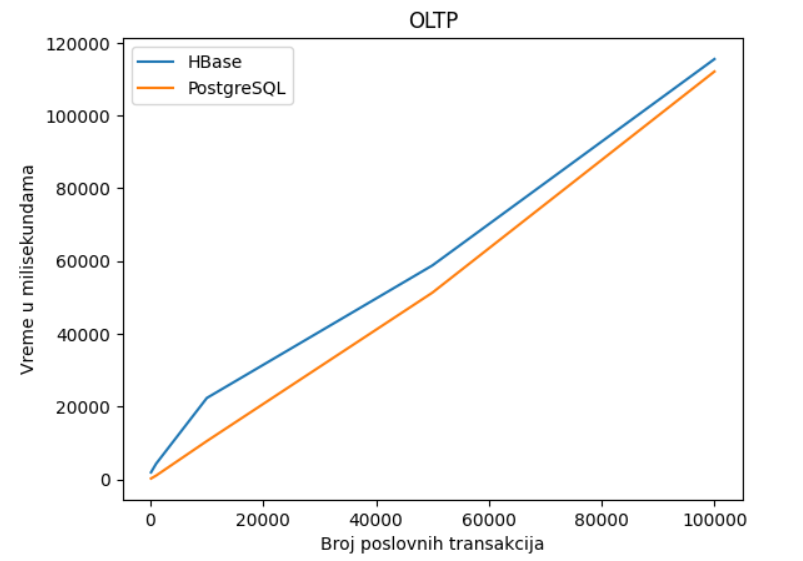
\includegraphics[width=0.8\textwidth]{oltp-vizualization.png}
  \caption{Rezultati merenja u OLTP okruženju}
  \label{fig:grafikon}
\end{figure}

\begin{figure}[!ht]
  \centering
  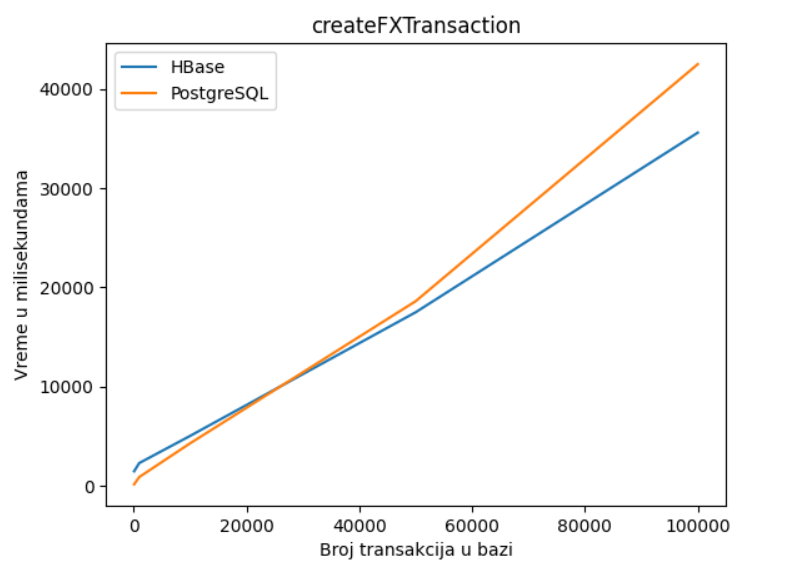
\includegraphics[width=0.8\textwidth]{createFxTransaction-vizualization.png}
  \caption{Rezultati merenja createFXTransaction dela poslovne transakcije}
  \label{fig:grafikon}
\end{figure}

\pagebreak 
\begin{figure}[!ht]
  \centering
  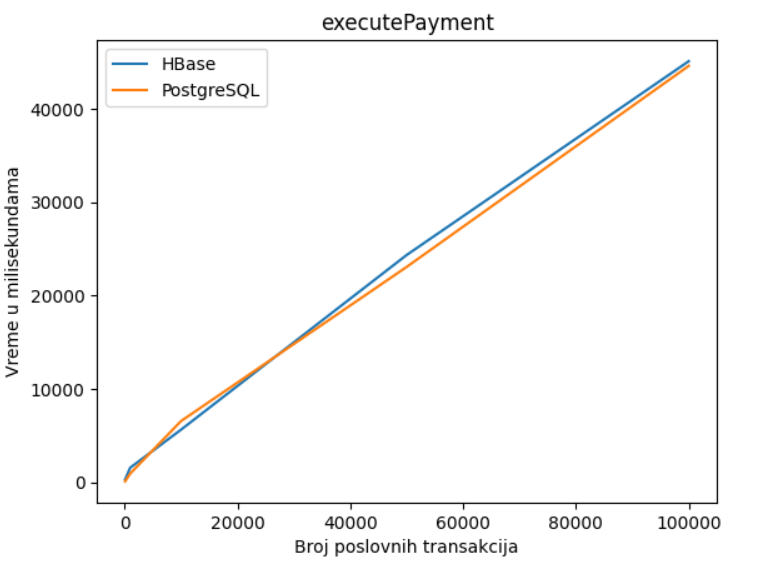
\includegraphics[width=0.8\textwidth]{executePayment-vizualization.png}
  \caption{Rezultati merenja executePayment dela poslovne transakcije}
  \label{fig:grafikon}
\end{figure}

\begin{figure}[!ht]
  \centering
  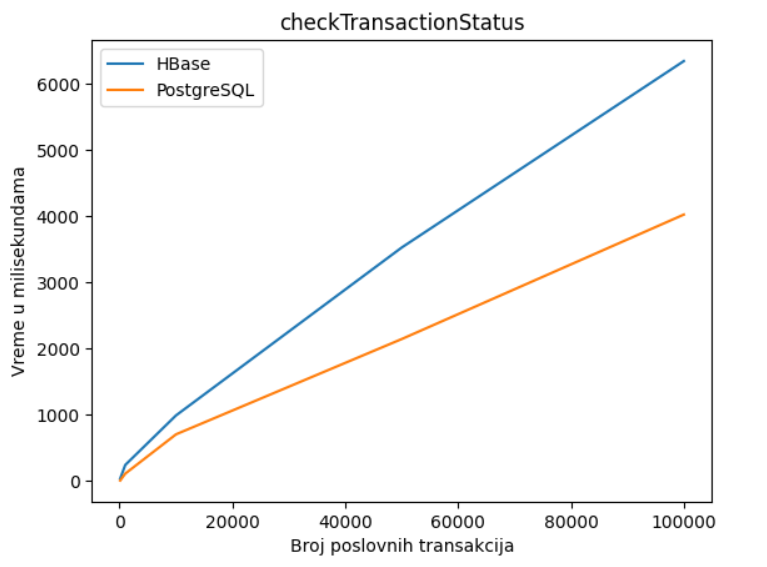
\includegraphics[width=0.8\textwidth]{checkTransactionStatus-vizualization.png}
  \caption{Rezultati merenja checkTransactionStatus dela poslovne transakcije}
  \label{fig:grafikon}
\end{figure}

\pagebreak

\section{Merenje performansi u OLAP okruženju}

Model baze podataka koji se koristi za testiranje u OLAP okruženju  sastoji se iz sledećih tabela:

\begin{enumerate}
\item[\textbullet] \textbf{product}: {
	Sadrži informacije o proizvodima. Sadrži \numprint{3000000} redova.
}
\item[\textbullet] \textbf{supplier}:{
	Podaci o dovaljačima. Sadrži  \numprint{1000000} redova.
}
\item[\textbullet] \textbf{productsupplier}:{
	Vezna tabela između dobavljača i proizvoda. Sadrži  \numprint{5000000} redova.
}
\item[\textbullet] \textbf{customer}:{
	Informacije o mušterijama. Sadrži  \numprint{1500000} redova.
}
\item[\textbullet] \textbf{order}:{
	Informacije o narudžbinama. Sadrži  \numprint{1500000} redova.
}
\item[\textbullet] \textbf{orderitem}:{
	Informacije o pojedinim stavkama narudžbine. Sadrži  \numprint{6000000} redova.
}
\end{enumerate}

\begin{lstlisting}[title={setup-postgres-model.sql - Kreiranje PostgreSQL modela},captionpos=b]
create table product (
    id  integer not null primary key,
    name varchar(50) not null,
    brand varchar(50) not null,
    type varchar(50) not null,
    size integer not null,
    container varchar(50) not null,
    price varchar(50) not null,
    comment varchar(50)
);

create table supplier (
    id  integer primary key,
    name varchar(50) not null,
    address varchar(200) not null,
    phone varchar(50) not null
);

create table productsupplier (
    id integer not null primary key,
    product integer not null,
    supplier integer not null,
    available integer not null,
    supply_cost real not null,
    comment varchar(200),
    constraint fk_product
    foreign key(product) references  postgresdb.product(id),
    constraint fk_supplier
    foreign key(supplier) references  postgresdb.supplier(id)
    
);

create table customer(
    id integer primary key,
    name varchar(50) not null,
    address varchar(200) not null,
    phone varchar(50) not null,
    comment varchar(200)
);

create table order(
    id integer primary key,
    customer integer not null,
    status varchar(20) not null,
    total_price real not null,
    entry_date date not null,
    priority varchar(20) not null,
    comment varchar(200),
    constraint fk_customer
    foreign key(customer) references  postgresdb.customer(id)
);

create table order_item(
    order_id integer not null,
    product integer not null,
    supplier integer not null, 
    order_no integer not null,
    quantity integer not null,
    base_price real not null,
    discount real not null,
    tax real not null,
    status varchar(20) not null,
    ship_date date not null,
    commit_date date not null,
    comment varchar(200),
    primary key(order_id,product,supplier),
    constraint fk_order
    foreign key(order_id) references  postgresdb.order(id),
    constraint fk_product
    foreign key(product) references  postgresdb.product(id),
    constraint fk_supplier
    foreign key(supplier) references  postgresdb.supplier(id)
);

\end{lstlisting}

\begin{lstlisting}[title={hbase-setup-model - Kreiranje HBase-a modela},captionpos=b]

create product, 'data';
create supplier, 'data';
create productsupplier, 'data';
create customer, 'data';
create order, 'data';
create orderitem, 'data';

\end{lstlisting}

OLAP test će obuhvatiti popunjavanje tabela iz csv fajlova (\textit{bulk load}), kao i iz izvršavanja upita koji će klijenti paralelno izvršavati više puta. Upit će biti parametrizovan i uzimaće dva parametra. Prvi parametar je dan narudžbine, a drugi je njen status. Na osnovu tih parametara dohvataju se agregirane vrednosti kolona iz tabele \textit{orderitem}, grupisane po statusu. 

\begin{lstlisting}[title={bulkLoad - Popunjavanje tabela iz csv fajlova},captionpos=b]
copy product from "./product.csv";
copy supplier from "./supplier.csv";
copy productsupplier "./productsupplier.csv";
copy customer from "./customer.csv";
copy order from "./order.csv";
copy order_item from "./order_item.csv";
\end{lstlisting}

\begin{lstlisting}[title={executeOLAPQuery - OLAP upit},captionpos=b]

select
	oi.status status,
	sum(oi.quantity) as sum_qty,
        sum(oi.base_price) as sum_base_price,
        sum(oi.base_price*(1-oi.discount)) as sum_disc_price,
        sum(oi.base_price*(1-oi.discount)*(1+oi.tax)) as sum_charge,
        avg(oi.quantity) as avg_qty,
        avg(oi.base_price) as avg_price,
        avg(oi.discount) as avg_disc,
        count(*) as count_order
from
         postgresdb.order_item oi
where
        oi.ship_date = to_date(?,'dd.mm.yyyy') and
         oi.status = ?
group by oi.status;
\end{lstlisting}


Parametri testa su \textbf{broj klijenata} (\textit{numOfClients}) koji će paralelno izvršavati olap upit i \textbf{ukupan broj izvršavanja upita} (\textit{totalIterations}). Oba parametra postavljaju se prilikom pokretanja testa, kroz standardni ulaz. Politika dodeljivanja broja izvršavanja upita svakom od klijenata ista je kao i dodeljivanja broja poslovnih transakcija klijentima, kod testiranja OLTP okruženja.

\begin{lstlisting}[title={Implementacija politike podele posla klijentima},captionpos=b]
List<Integer> iterClientList = new ArrayList<>();
int itersToAssign = totalIterations;
int itersPerClient = itersToAssign / numOfClients;

for(int i = 0; i<numOfClients;i++){	
   iterClientList.add(itersPerClient);
   itersToAssign-=itersPerClient;
}
if (itersToAssign > 0) {
   int itersForLast = iterClientList.get(numOfClients - 1);
   iterClientList.set(numOfClients - 1, itersForLast + itersToAssign);
}
assert numOfClients==iterClientList.size();
Thread[] threads = new Thread[numOfClients];
for(int i = 0;i<numOfClients;i++){
   threads[i] = new Thread(
      new BenchmarkSingleClientExecutor(
         i*iterClientList.get(i),iterClientList.get(i)
         )
      );
}
\end{lstlisting}

Svaki klijent nakon što mu je dodeljen broj iteracija, kreće da izvršava upit onoliko puta koliko mu je iteracija dodeljeno. Svako izvršavanje OLAP upita ima iste parametre.


\begin{lstlisting}[title={BenchmarkSingleClientExecutor.java - Posao klijenta},captionpos=b]
public class BenchmarkSingleClientExecutor implements Runnable {

private final CountDownLatch endSignal;
private final BenchmarkOLAPUtility olapUtil;
private final int numOfIters;
private final int start;

private final Object connection;
@Override
public void run() {
  try {
    for (int i = this.start; i < this.start + this.numOfIters; i++) {
       olapUtil.executeOLAPQuery(connection);
     }
     endSignal.countDown();
    } catch (Throwable e) {
      throw new IllegalStateException(e);
    }
  }
}
\end{lstlisting}

Priprema okruženja za testiranje podrazumeva generisanje csv fajlova koji kasnije treba da budu učitani u tabele koristeći podršku za \textit{bulk load}, zatim kompilaciju java testova, pokretanje docker kontejnera i prebacivanje kompiliranih testova kao i izgenerisanih csv fajlova na odgovarajuće kontejnere. Dodatan korak za HBase jeste da se na HBase kontejneru kreira struktura baze podataka. Skripta u nastavku sadrži sve neophodne komande za pokretanje okruženja.

\begin{lstlisting}[title={prepareEnv.sh - Skripta za pokretanje OLAP okruženja},captionpos=b]
#!/bin/bash
echo 'PREPARING ENVIRONMENT...';
echo 'PREPARING HBASE BENCHMARK JARS...';
export JAVA_HOME="$JAVA_8";
mvn -f olap_benchmark_hbase clean compile assembly:single;
mvn -f hbase_setup_olap_model clean compile assembly:single;
mvn -f hbase_bulk_load_setup clean compile assembly:single;

echo 'PREPARING HBASE BULK LOAD RESOURCES..';
java -jar ./hbase_bulk_load_setup.jar;


echo 'PREPARING POSTGRES BENCHMARK JARS...';
export JAVA_HOME="$JAVA_17";
mvn -f olap_benchmark_postgres clean compile assembly:single;
mvn -f postgres_bulk_load_setup clean compile assembly:single;

echo 'PREPARING POSTGRES BULK LOAD RESOURCES..';
java -jar postgres_bulk_load_setup.jar;

docker-compose -f docker-compose.yml up --build -d;
winpty docker exec -it hbase sh -c "java -jar setup_olap_model.jar";
\end{lstlisting}


\begin{lstlisting}[title={docker-compose.yml - Definicija kontejnera za OLAP okruženje},captionpos=b]

services: 
  postgres:
    container_name: postgres
    ports:
      - "5433:5432"
    volumes:
      - ./setup_model.sql:/docker-entrypoint-initdb.d/create_script.sql
      - ./benchmark_postgres.jar:/benchmark_postgres.jar
    environment:
      - POSTGRES_PASSWORD=postgres
      - POSTGRES_USER=postgres
      - POSTGRES_DB=postgresdb
    build:
      context: .
      dockerfile: ./Dockerfile_postgres

  hbase:
    image: bde2020/hbase-standalone:1.0.0-hbase1.2.6
    container_name: hbase
    volumes:
      - ./productsupplierHB.csv:/productsupplier.csv
      - ./productHB.csv:/product.csv
      - ./supplierHB.csv:/supplier.csv
      - ./customerHB.csv:/customer.csv
      - ./orderHB.csv:/order.csv
      - ./orderitemHB.csv:/orderitem.csv
      - ./orderitemStatsHB.csv:/orderitemstats.csv
      - hbase_data:/hbase-data
      - hbase_zookeeper_data:/zookeeper-data
      - ./hbase_setup_model.jar:/hbase_setup_model.jar
      - ./benchmark_hbase.jar:/benchmark_hbase.jar
    ports:
      - 16000:16000
      - 16010:16010
      - 16020:16020
      - 16030:16030
      - 2888:2888
      - 3888:3888
      - 2181:2181

volumes:
  hbase_data:
  hbase_zookeeper_data:
\end{lstlisting}

Rezultati merenja prikazani u nastavku nastali kao rezultat pokretanja testova sa \numprint{10}, \numprint{20}, \numprint{50}, \numprint{100} iteracija izvršavanja OLAP upita i pet klijenata koji te upite paralelno izvršavaju.

\begin{figure}[!ht]
  \centering
  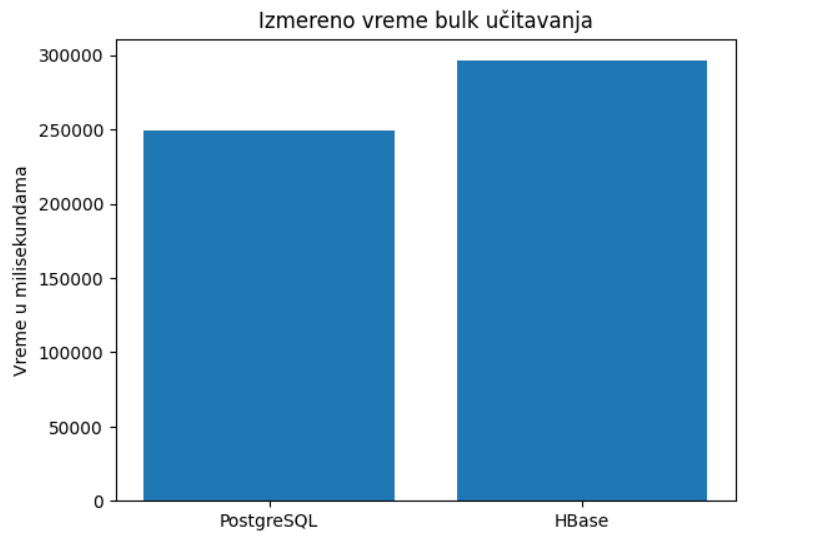
\includegraphics[width=0.8\textwidth]{bulk-load-vizualization.png}
  \caption{Bulk load podataka}
  \label{fig:grafikon}
\end{figure}

\begin{figure}[!ht]
  \centering
  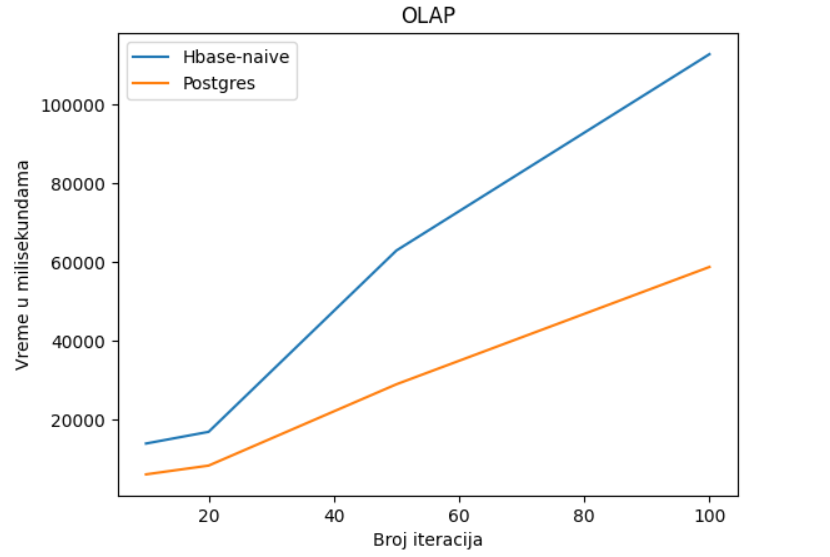
\includegraphics[width=0.7\textwidth]{olap-vizualization2.png}
  \caption{OLAP}
  \label{fig:grafikon}
\end{figure}



\section{Merenje performansi u distribuiranom okruženju}

Kao što je napomenuto u 3.3 za merenje performansi koriste se OLTP i OLAP testovi iz poglavlja 3.1 i 3.2. Jedina razlika će biti priprema okruženja za testiranje. 
U ovom slučaju testiranje se izvršava na fizičkom čvoru (računaru) sa 10 procesorskih jezgara, stepenom mulitprocesiranja 12 i ranije instaliranim HBase-om i Hadoop-om. 

Priprema okruženja podrazumeva najpre pokretanje HDFS klastera, koji se sastoji iz jednog HDFS master čvora i jednog HDFS čvora podataka, sa postavljenim faktorom replikacije blokova:

\begin{lstlisting}[title={start-hadoop.sh - Komande za pokretanje HDFS komponenti},captionpos=b]
#!/bin/bash
$HADOOP_HOME/sbin/start-dfs.sh
$HADOOP_HOME/sbin/start-yarn.sh
\end{lstlisting}

\begin{lstlisting}[title={hdfs-site.xml - Konfiguracija HDFS-a sa faktorom replikacije 2},captionpos=b]
<configuration>
      <property>
	<name>dfs.replication</name>
          <value>2</value>
      </property>
      <property>
  	<name>dfs.datanode.data.dir</name>
  	<value>/home/lukadj/hadoop/data2</value>
      </property>
</configuration>
\end{lstlisting}

Nakon toga pokreće se HBase klaster koji se sastoji iz jednog region servera, jednog master servera i zookeeper servisa. HBase je konfigurisan tako da koristi ranije pokrenut HDFS klaster.

\begin{lstlisting}[title={start-hbase.sh - Komanda za pokretanje HBase-a},captionpos=b]
#!/bin/bash
$HBASE_HOME/bin/start-hbase.sh
\end{lstlisting}

\pagebreak

\begin{lstlisting}[title={hbase-site.xml - Konfiguracija distribuiranog HBase-a},captionpos=b]
 <property>
    <name>hbase.cluster.distributed</name>
    <value>true</value>
  </property>
  <property>
    <name>hbase.rootdir</name>
    <value>hdfs://localhost:9000/hbase</value>
  </property>
  <property>
    <name>hbase.zookeeper.property.clientPort</name>
    <value>10231</value>
  </property>
\end{lstlisting}


\begin{figure}[!ht]
  \centering
  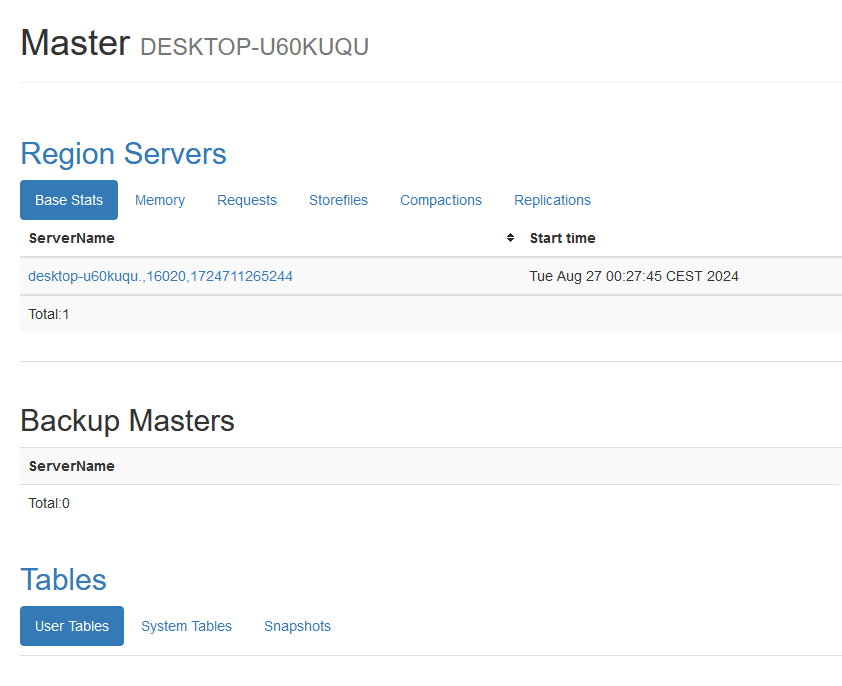
\includegraphics[width=0.9\textwidth]{hbase-master.png}
  \caption{Stranica za praćenje hbase master servera}
  \label{fig:grafikon}
\end{figure}

\pagebreak


\begin{figure}[!ht]
  \centering
  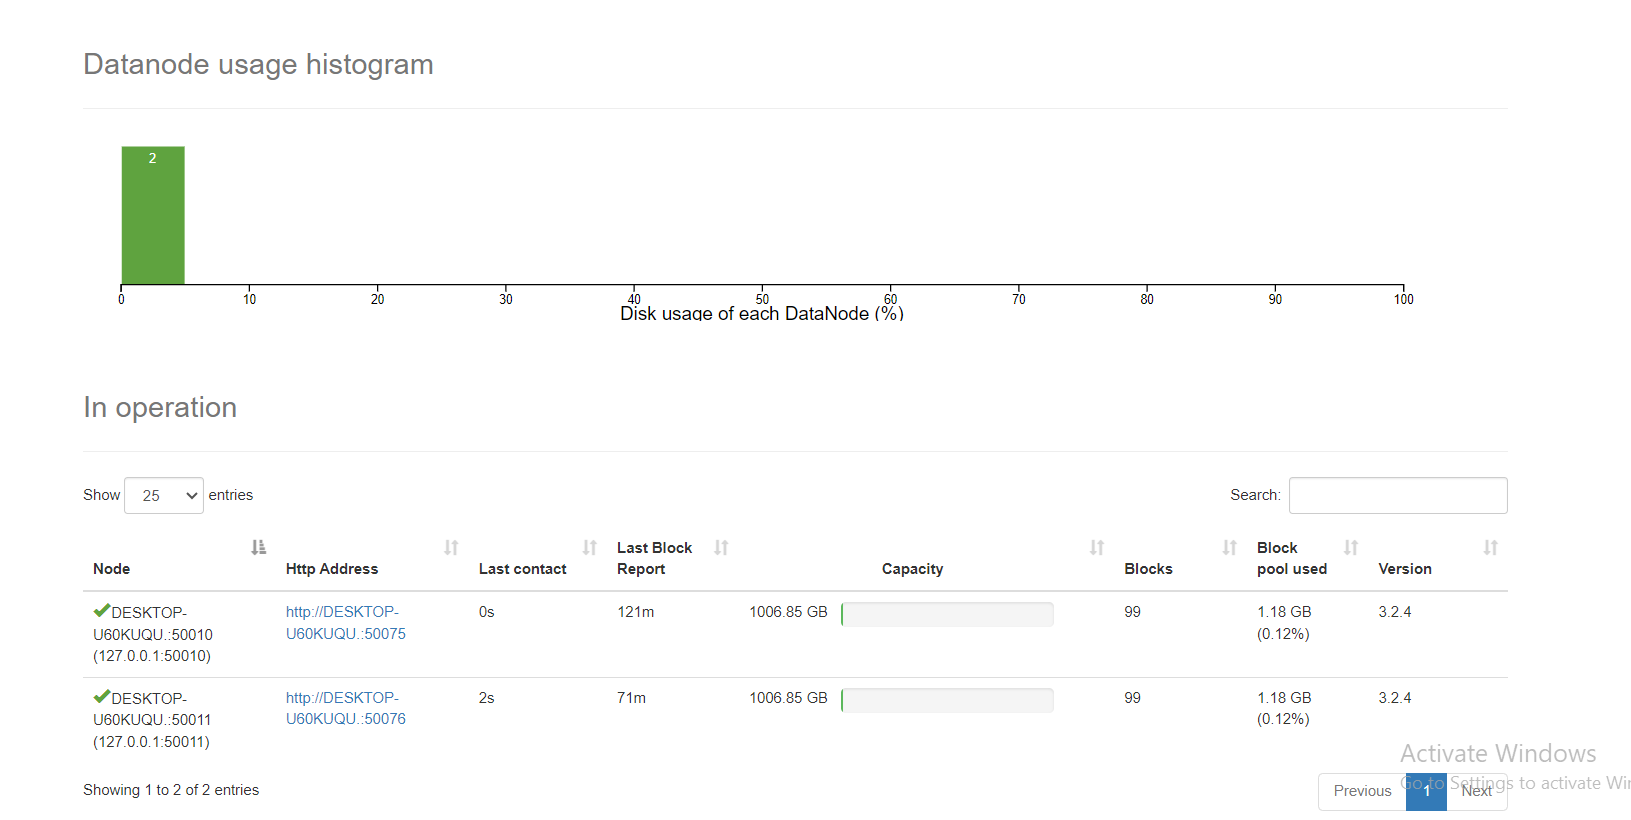
\includegraphics[width=0.9\textwidth]{datanode.png}
  \caption{Stranica za praćenje HDFS čvorova podataka}
  \label{fig:grafikon}
\end{figure}


Poređenje rezultata merenja distribuiranog HBase klastera sa nedistribuiranim HBase-om  prikazano u nastavku nastalo je kao rezultat pokretanja OLTP testova sa \numprint{100}, \numprint{1000}, \numprint{10000}, \numprint{50000}, \numprint{100000} poslovnih transakcija.

\begin{figure}[!ht]
  \centering
  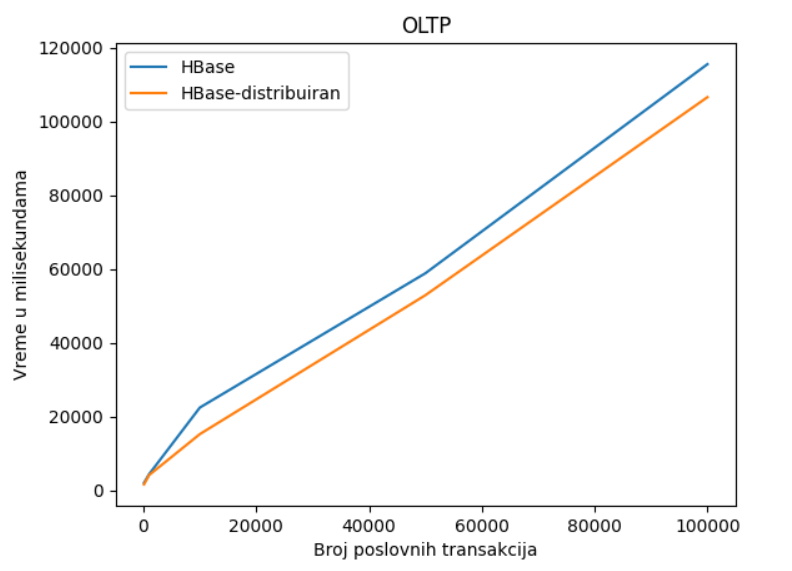
\includegraphics[width=0.7\textwidth]{dist-results.png}
  \caption{Upoređivanje rezultata dobijenih u OLTP okruženju za distribuirani i nedistribuirani HBase}
  \label{fig:grafikon}
\end{figure}

\pagebreak

Poređenje rezultata merenja distribuiranog HBase klastera sa nedistribuiranim HBase-om prikazano u nastavku nastalo je kao rezultat pokretanja OLAP testova sa \numprint{10}, \numprint{20}, \numprint{50}, \numprint{100} iteracija.

\begin{figure}[!ht]
  \centering
  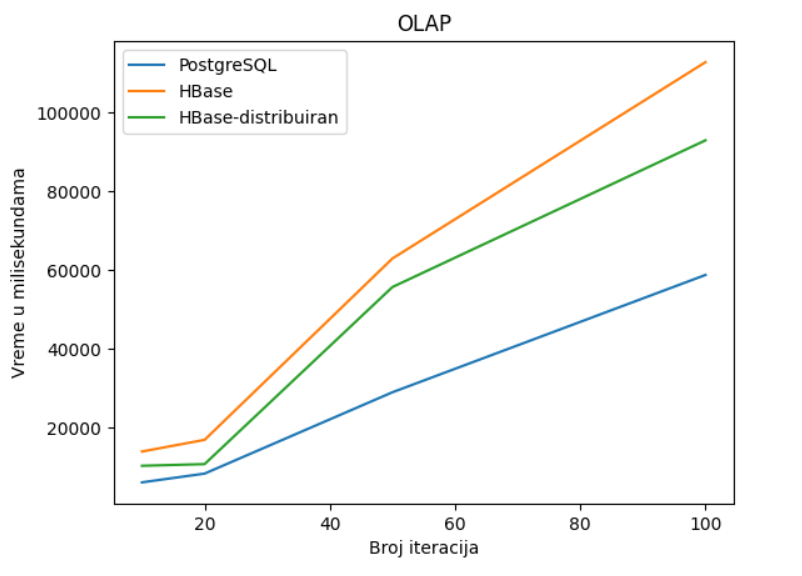
\includegraphics[width=0.7\textwidth]{dist-olap.png}
  \caption{Upoređivanje rezultata dobijenih u OLAP okruženja za distribuirani i nedistribuirani HBase }
  \label{fig:grafikon}
\end{figure}



\chapter{Analiza rezultata}

Analiza rezultata obuhvata interpretaciju rezultata koji su dobijeni merenjima performansi, kao i navođenje eventualnih unapređenja i primedbi koje treba imati u vidu kada se radi sa datim tehnologijama.

\section{Analiza rezultata kod testiranja u OLTP okruženju}

Rezultati merenja ukazuju da kako raste broj poslovnih transakcija koje treba obraditi u testu, inicijalna prednost PostgreSQL-a u odnosu na HBase opada. Konkretno po fazama poslovne transakcije, izdvaja se createFXTransaction transakcija baze podataka, kod koje na postavljenih 50000 i 100000  poslovnih transakcija, HBase ima prednost. Sa druge strane, na primeru \textit{checkTransactionStatus}-a vidi se da pretraga po primarnom ključu kod PostgreSQL-a radi brže nego što je to slučaj kod HBase-a.  I pored toga ukupni rezultati ukazuju na tendenciju da bi sa porastom broja poslovnih transakcija (na milion ili deset miliona) PostgreSQL imao veća usporenja, relativno u odnosu na HBase, međutim za testiranje takvog okruženja neophodno je koristiti računar koji je sposoban da sprovede tako zahtevan test.

Važno je naglasiti da HBase ne garantuje konzistentost nad svim podacima kakvu nudi PostgreSQL. HBase nudi jedan vid konzistenosti, i to konzistetnost u radu sa jednom redom tabele (više o tome u 2.2). To dovodi do zaključka da ukoliko je neophodno implementirati transakciju koja uključuje rad sa podacima više tabela ili više redova jedne tabele, ukoliko koristimo HBase, moramo na aplikativnom sloju voditi računa o očuvanju  eventualne konzistetnosti. PostgreSQL sa druge strane kao ACID baza podataka, sama garantuje konzistentost, te ne zahteva dodatan napor kao u slučaju HBase-a. 

\section{Analiza rezultata kod testiranja u OLAP okruženju}

Rezultati merenja u okviru OLAP rezultata ističu prednost PostgreSQL-a u performansama. Prednost HBase-a u odnosu na PostgreSQL jeste fleksiblnost sheme koja u ovakvom slučaju može doći do izražaja. Dorada modela koja se u slučaju HBase-a može primeniti može doneti dramatična poboljšanja u performansama čitanja HBase-a čak i u odnosu na PostgreSQL. 

Kreiranje tabele (u ovom slučaju orderitemstats) koja za vrednost ključa ima status, a za kolone ima vrednosti svake potrebne agregirane funkcije po danima, uticalo bi na to da se čitanje izveštaja svodi na čitanje po ključu sa izdvajanjem potrebnih koloni\footnote{ Razlog zašto se ovakva modifikacija ne može primeniti u slučaju PostgreSQL-a jeste ograničen broj kolona, kao i to što skup kolona mora biti unapred definisan pri kreiranju modela. Kod HBase-a takvi limiti ne postoje.}.
Primer dodate tabele može se videti na slici 5.1 ,a uticaj na performanse na slici 5.2.

\begin{figure}[!ht]
  \centering
  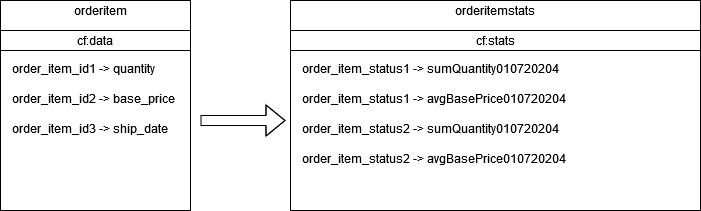
\includegraphics[width=1\textwidth]{denormalized-model.png}
  \caption{Tabela orderitemstats}
  \label{fig:grafikon}
\end{figure}

\begin{figure}[!ht]
  \centering
  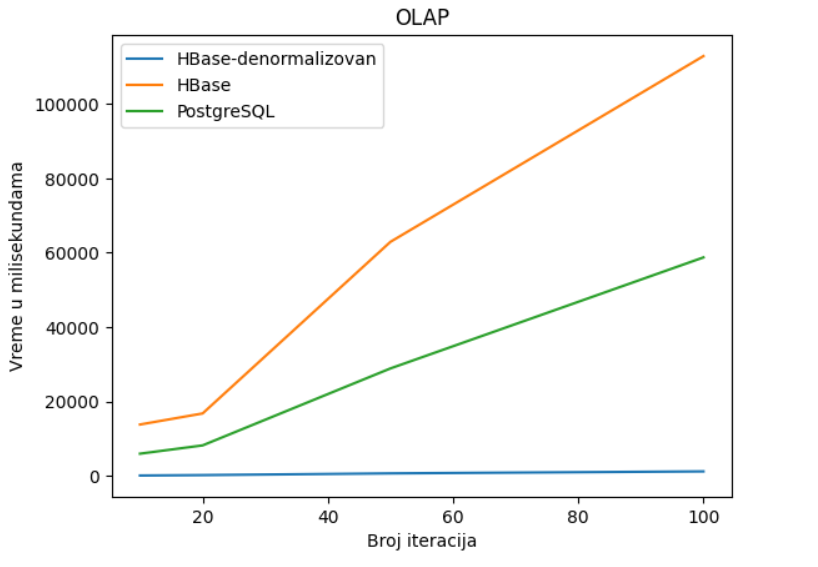
\includegraphics[width=0.8\textwidth]{olap-vizualization.png}
  \caption{Uporedna analiza performansi PostgreSQL-a i HBase-a}
  \label{fig:grafikon}
\end{figure}

Sa druge strane PostgreSQL takođe podržava mehanizme koji u ovom slučaju mogu poboljšati performanse. Konkretno za ovaj test, možemo kreirati materijalizovani pogled \textit{mv\_order\_item\_bydate} sa rezultatima ranije izračunatih statističkih funkcija. Tada bi se OLAP upit iz testa pretvorio u čitanje podataka iz materijalizovanog pogleda umesto izračunavanja agregiranih funkcija. Takva optimizacija ima veliki uticaj na performanse, slika 5.3.

\pagebreak 

\begin{lstlisting}[title={mvorder\_item\_bydate - Kreiranje materijalizovanog pogleda},captionpos=b]
create materialized view  postgresdb.mvorder_item_bydate
    as (select
	  oi.ship_date,
	  sum( oi.quantity ) as sum_qty,
	  sum(OI.BASE_PRICE) as sum_base_price,
	  sum(OI.BASE_PRICE*(1-OI.discount)) as sum_disc_price,
	  sum(OI.BASE_PRICE*(1-OI.discount)*(1+OI.TAX)) as sum_charge,
	  avg(OI.QUANTITY) as avg_qty,
	  avg(OI.BASE_PRICE) as avg_price,
	  avg(OI.DISCOUNT) as avg_disc,
	  count(*) as count_order
	  from postgresdb.order_item oi
	  group by oi.status, oi.ship_date)
	with data;
 \end{lstlisting}

\begin{lstlisting}[title={executeOLAPQuery - OLAP upit koristeći materijalizovani pogled},captionpos=b]
select *
	from postgresdb.mv_order_item_bydate
        where ship_date = TO_DATE(?,'DD.MM.YYYY')
	and status = ?
 \end{lstlisting}


\begin{figure}[!ht]
  \centering
  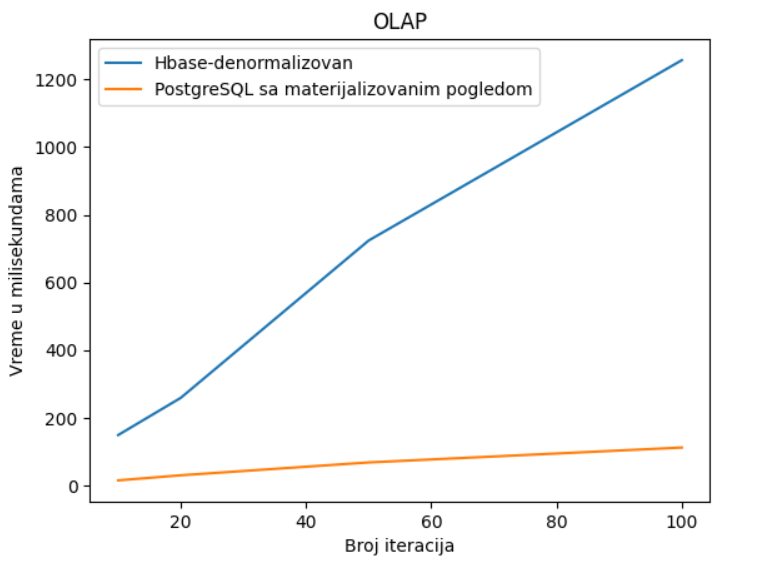
\includegraphics[width=0.8\textwidth]{mv-denormalizerd.png}
  \caption{Uporedna analiza performansi koristeći optimizaciju kod HBase-a  i PostgreSQL-a}
  \label{fig:grafikon}
\end{figure}


\section{Analiza rezultata kod testiranja u distribuiranom okruženju}

Analiza rezultata testiranja u distribuiranom okruženju obuhvatiće uporednu analizu sa nedistribuiranim HBase-om, opis fragmentacije i replikacije podataka kao i organizacije podataka HBase-a na HDFS čvoru. 

Pokrenuti distribuirani HBase klaster pokazuje nešto bolje rezultate nego nedistribuirani HBase koji podatke skladišti na lokalnom fajl sistemu. Jedan od razloga za to je integracija HBase baze podataka sa HDFS ekosistemom\cite{hbaseGuide}.  Drugi razlog boljih performansi u odnosu na nedistribuirani HBase može biti i to što se pri nedistribuiranom izvršavanju potencijalno ne koriste sva jezgra fizičkog čvora, pa se pri distribuiranju u više procesa na istom fizičkom čvoru povećava iskorišćenost procesora. Merenje iskorićenosti procesora (\textit{CPU}\%) u nedistribuiranom i distribuiranom okruženju sa jednim region server čvorom dalo je manju prednost distribuiranom, slika 5.4 i 5.5. 

\begin{figure}[!ht]
  \centering
  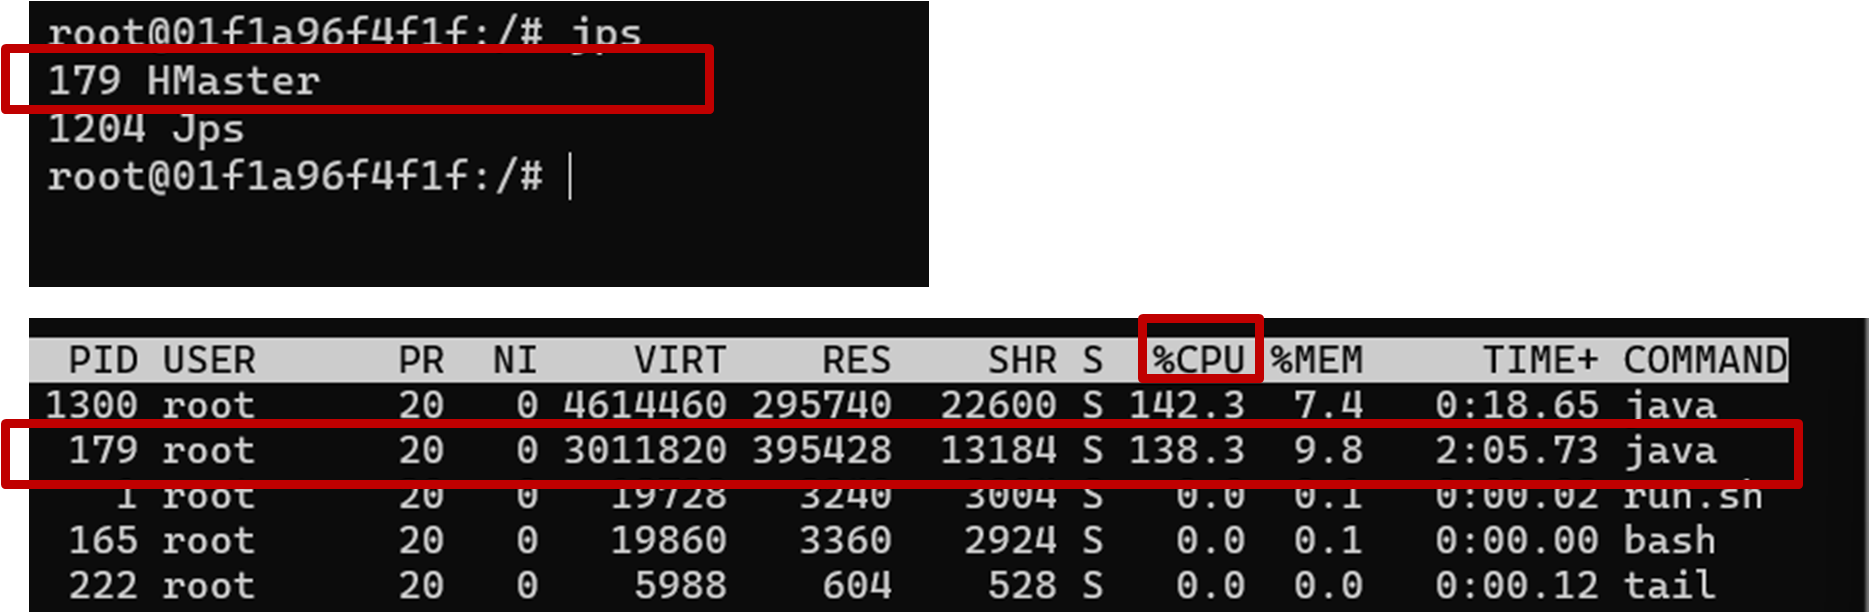
\includegraphics[width=1\textwidth]{nedistribuiro-cpu.png}
  \caption{Iskorišćenost procesora u nedistribuiranom okruženju}
  \label{fig:grafikon}
\end{figure}


\begin{figure}[!ht]
  \centering
  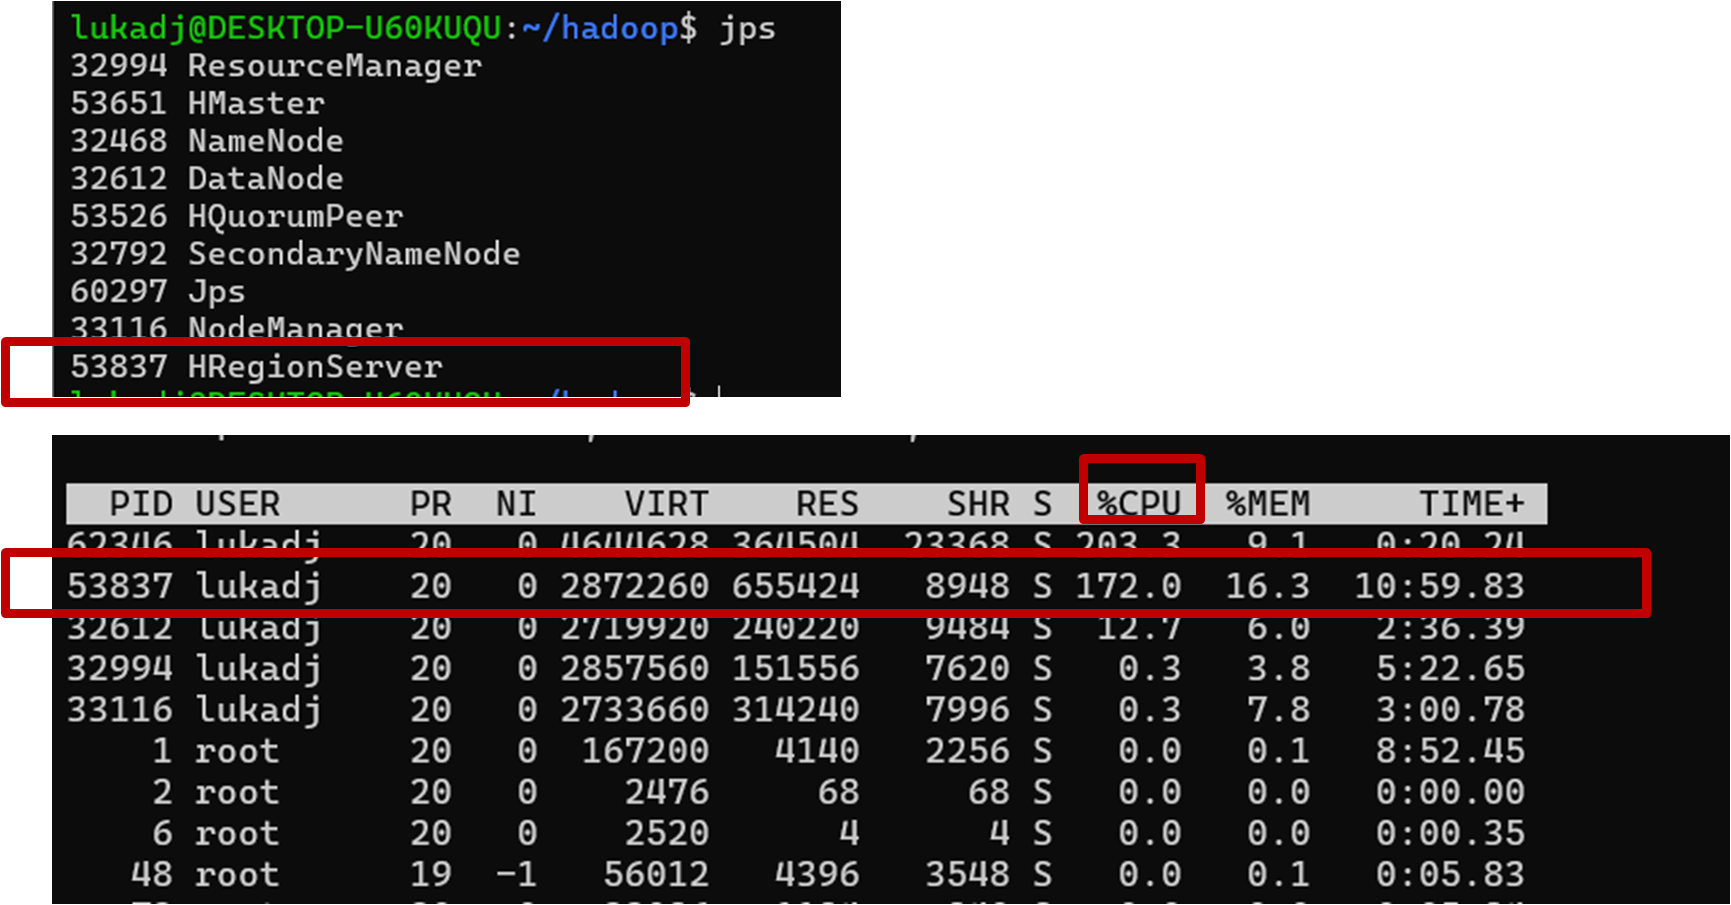
\includegraphics[width=1\textwidth]{distribuirano-cpu.png}
  \caption{Iskorišćenost procesora u distribuiranom okruženju}
  \label{fig:grafikon}
\end{figure}

\pagebreak 
Ograničenje ove studije je korišćenje jednog fizičkog čvora sa jednim region server čvorom. Sa povećanjem broja region servera na istom fizičkom čvoru potencijalno bi se postigla veća iskorišćenost procesora, a samim tim i bolje performanse, što može biti predmet daljih istraživanja. Povećavanjem broja fizičkih čvorova postigla bi se veća pouzdanost klastera, bolja dostupnost i brže čitanje podataka \cite{ColumnarOriented}.  

Fragmentacija HBase klastera realizovana je na dva nivoa:  fragmentacija odgovornosti region servera za regione koji mogu pripadati različitim tabelama i fragmentacija podataka u okviru HDFS klastera. Sa druge strane replikacija je prisutna samo za podatke u okviru HDFS klastera, ali ne i u odgovornosti region servera, jer je za jedan region u svakom trenutku odgovoran samo jedan region server.

Na slici 5.6. prikazana  je organizacija regiona (kolone \textit{Regions}) po tabelama (kolona \textit{Name}) kojima pripadaju. Broj regiona srazmeran je broju redova tabele, odnosno količini podataka koje tabela sadrži. 

\begin{figure}[!ht]
  \centering
  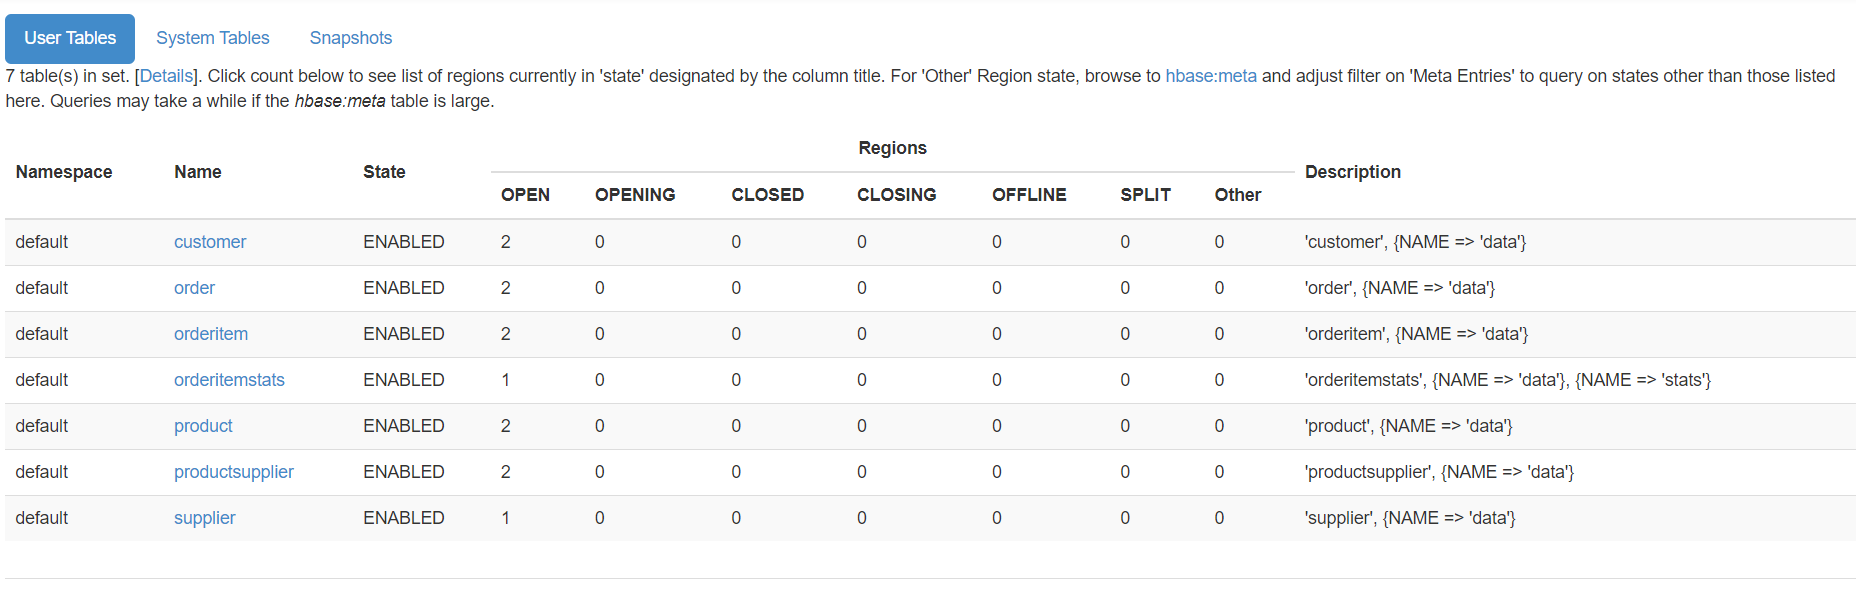
\includegraphics[width=1\textwidth]{master-dist.png}
  \caption{Organizcija regiona po tabelama kojima pripadaju}
  \label{fig:grafikon}
\end{figure}

Lista regiona, njihovi opsezi, kao i veličine mogu se videti na  primeru tabele orderitem, na slici 5.7.

\begin{figure}[!ht]
  \centering
  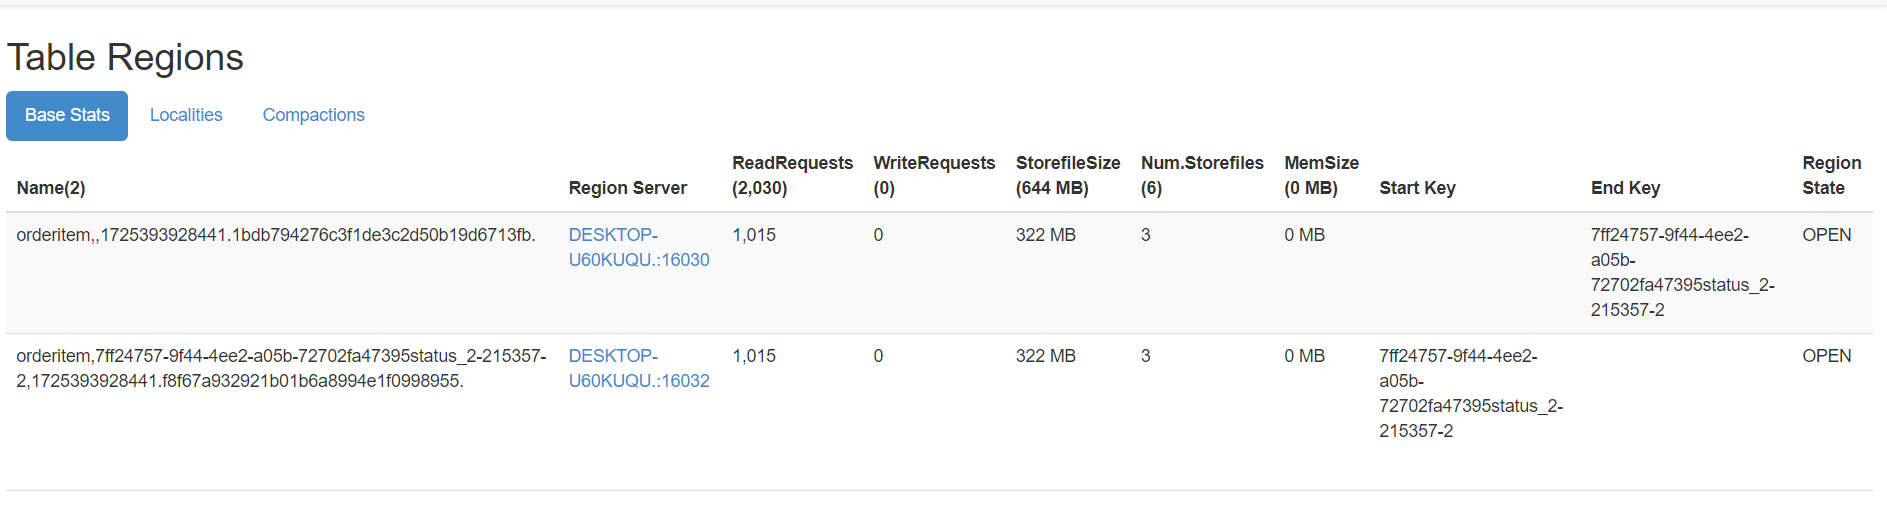
\includegraphics[width=1\textwidth]{orderitem-regions.png}
  \caption{Regioni tabele orderitem}
  \label{fig:grafikon}
\end{figure}


Na HDFS čvoru podaci su organizovani tako da svaka tabela ima svoj direktorijum\footnote{Direktorijum ne predstavlja fizičku lokaciju na jednom HDFS čvoru, jer regioni jedne HBase tabele mogu biti čuvani na više HDFS čvorova.}, slika 5.8.

Svaki region je u okviru HDFS klastera fragmentisan na blokove, koji su replikovani u skladu sa vrednošću faktora replikacije klastera (\textit{Replication}), slika 5.9.

\begin{figure}[!ht]
  \centering
  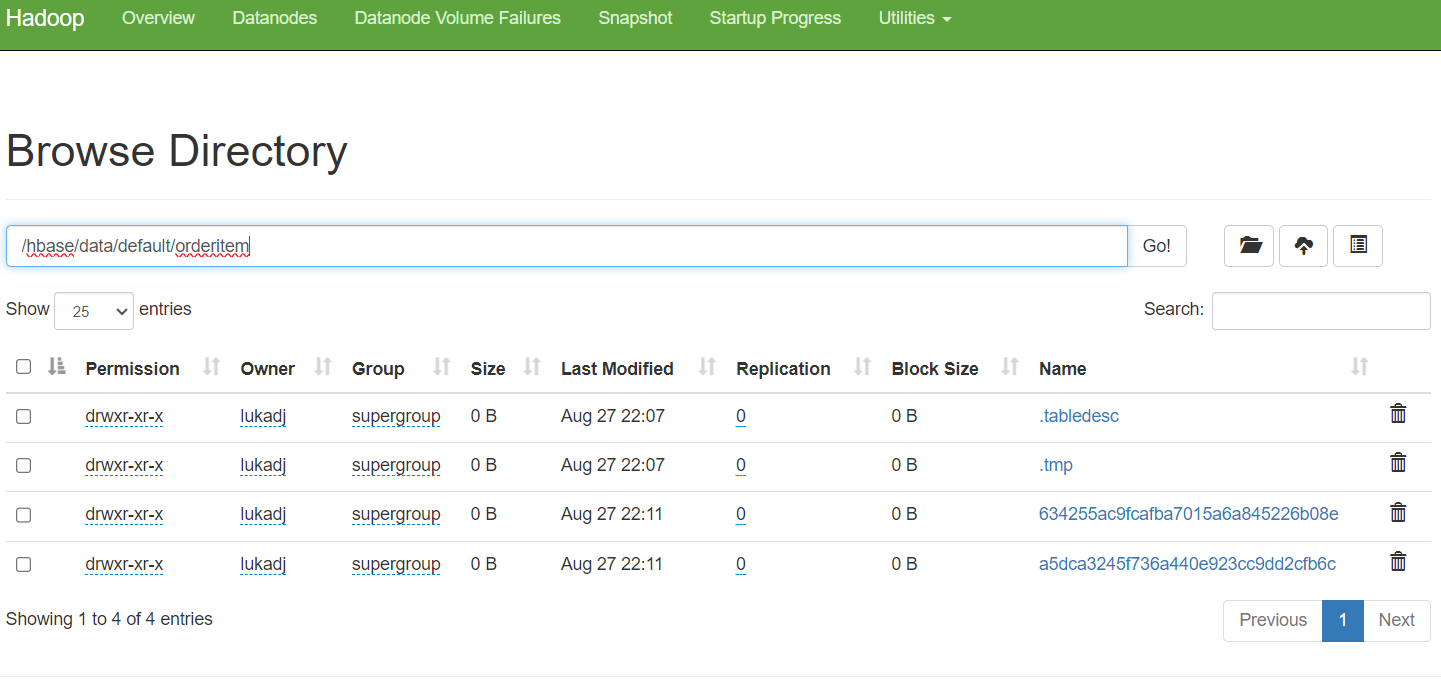
\includegraphics[width=1\textwidth]{orderitem-datanode.png}
  \caption{Orderitem direktorijum na HDFS čvoru sadrži regione u vidu poddirektorijuma}
  \label{fig:grafikon}
\end{figure}

\begin{figure}[!ht]
  \centering
  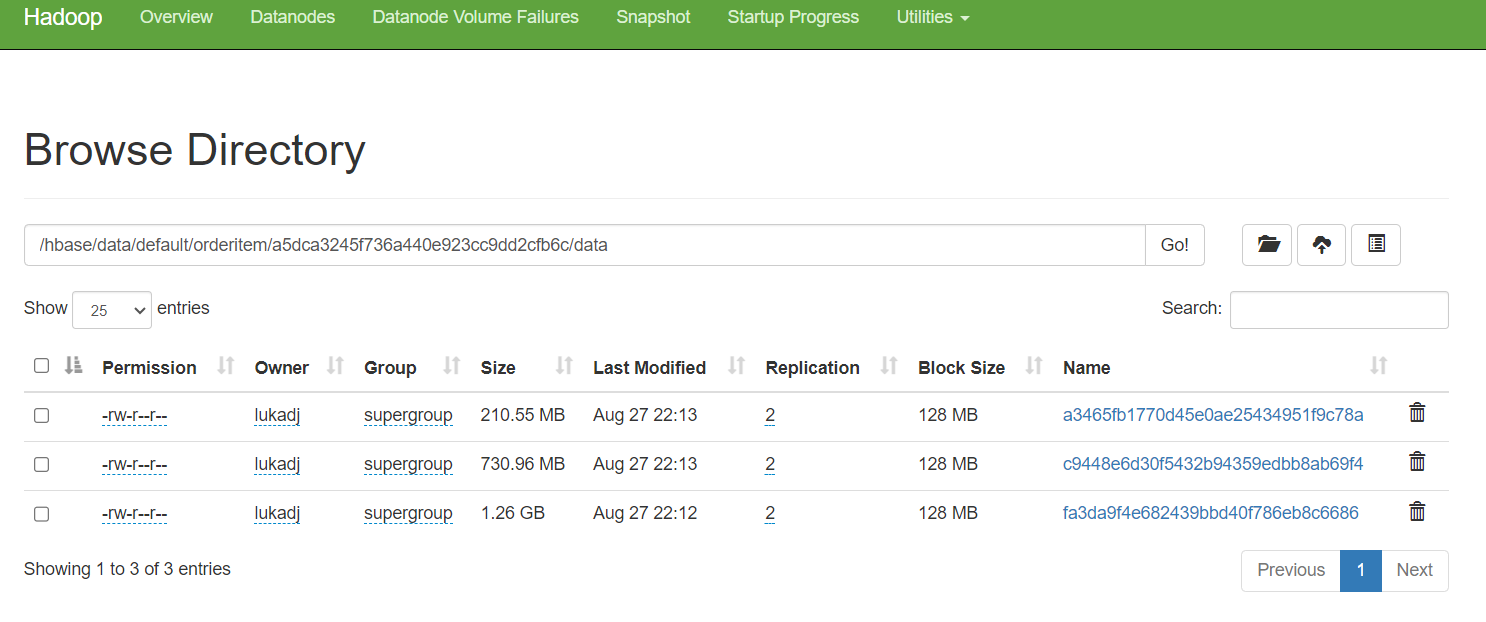
\includegraphics[width=1\textwidth]{orderitem-datanode-regions-blocks.png}
  \caption{Region je na HDFS čvoru interno podeljen na blokove}
  \label{fig:grafikon}
\end{figure}




\chapter{Zaključak}

U ovom radu su opisani relacioni i kolonski orijentisani modeli baza podataka kao i glavne razlike između njih. U svrhu testiranja izabrana su i opisana dva predstavnika odgovarajućih modela: PostgreSQL kao predstavnik relacionih baza podataka i HBase kao predstavnik kolonski orijentisanih baza podataka.

Kako bi se postigao dovoljan dokaz koncepta, simulirana su različita okruženja sa posebnim modelima i namenama i to: OLTP okruženje, OLAP okruženje i distribuirano okruženje.

Analiza rezultata merenja u OLTP okruženju pokazala je da u performansama nad ograničenim brojem podataka nema velike razlike između HBase-a i PostgreSQL-a, uz prepoznavanje tendencije da sa porastom broja podataka HBase ima manja usporenja nego PostgreSQL. Sa druge strane PostgreSQL nudi ACID garancije kakve kod HBase-a nemamo, i ukoliko ih želimo, moramo ih obezbediti na aplikativnom sloju.

Analiza rezultata merenja u OLAP okruženju, pokazala nam je da PostgreSQL ima prednost pri izvršavanju složenih upita koji pored prostog čitanja podataka sadrže i operacije nad podacima (npr. računanje sume, proseka itd). Fleksibilnost strukture kod HBase-a daje nam prostor da performanse unapredimo, kreirajući tabelu koja sadrži ranije izračunate agregirane vrednosti. Međutim još bolji efekat se može postići kod PostgreSQL-a kreiranjem materijalizovanog pogleda, što je u radu i prikazano.

Analiza distribuiranog okruženja obuhvatila je opis organizacije podataka na HBase klasteru kao i upoređivanje tipova distribuiranosti PostgreSQL-a i HBase-a, na osnovu teorijskih izvora. Usled složenosti imlementacije, nedostaje implementacija testa koji radi sa distirbuiranim PostgreSQL klasterom tako da je ovaj segment rada ograničen na implementaciju samo HBase klastera. Data je analiza tipova replikacija koje koriste HBase i PostgreSQL  u distribuiranom okruženju i istaknute su prednosti i mane svakog od njih.

% S obzirom da HBase za distribuiranje koristi replikaciju bez master servera koju je (koju je nasledio od HDFS-a) nudi visok nivo otpornosti na greške kao i dostupnosti klastera. Sa druge strane PostgreSQL (a i ostale relacione baze podatka) koriste master-slave replikaciju, i to najčešće %njen sinhroni oblik, on nudi visok nivo 

Teorijska analiza i analiza merenja rezultata pokazala je primere primene HBase-a i PostgreSQL-a. Ukoliko radimo sa \textbf{velikom} količinom \textbf{slabo struktuiranih} podataka koji rade na \textbf{nepouzdanim} serverima, gde ima velike količine \textbf{pisanja} podataka, a operacije čitanja su pretežno \textbf{po ključu} ili \textbf{njegovom prefiksu} \footnote{U 5.2. prikazan je primer kako uvođenje tabele u modelu može dovesti do svođenja složenih upita na čitanje po ključu}, nameće se HBase kao bolji izbor tehnologije koja će upravljati podacima. Ukoliko radimo sa \textbf{ograničenom} količinom \textbf{struktuiranih} podataka, koji će se obrađivati na \textbf{pouzdanim} serverima, PostgreSQL je bolje rešenje.

Možemo zaključiti da nijedna od tehnologija ne predstavlja univerzalno rešenje, i da svaka od njih ima svoje mesto za primenu, kao i da je za odabir pogodnog sistema za upravljanje podacima neophodno postojanje testova koji pokrivaju što veći skup slučajeva upotrebe. Ovaj rad predstavlja bazu platforme za testiranje slučajeva upotrebe, tako da se skup slučajeva upotrebe može proširivati i na taj način obogatiti.



%U radu je dat opis relacionog kao i kolonski orijentisanog nerelacionog modela, uz to i opis PostgreSQL-a i HBase-a kao njihovih predstavnika. Centralni deo rada predstavlja analiiza slučajeva upotrebe, što kroz implementirane testove, što kroz 
% ------------------------------------------------------------------------------
% Literatura
% ------------------------------------------------------------------------------
\literatura

% ==============================================================================
% Završni deo teze i prilozi
\backmatter
% ==============================================================================

% ------------------------------------------------------------------------------
% ------------------------------------------------------------------------------

\end{document} 